\documentclass[11pt, a4paper]{article}
\usepackage[a4paper, margin=2.2cm]{geometry}
\usepackage{fontspec}
\usepackage[english, provide=*]{babel}
\babelprovide[import, onchar=ids fonts]{english}
\IfFontExistsTF{Arial}{\babelfont{rm}{Arial}}{\babelfont{rm}{DejaVu Sans}}
\usepackage{amsmath, amssymb}
\usepackage{booktabs}
\usepackage{tabularx}
\usepackage{array}
\usepackage{graphicx}
\usepackage[hidelinks]{hyperref}
\usepackage{algorithm}
\usepackage{algpseudocode}

\setlength{\parskip}{0.45em}
\setlength{\parindent}{0pt}

\title{\textbf{Deep Physics-Guided Alternating Activity and Attenuation Reconstruction for CT-less Quantitative Bone SPECT with Differentiable Distance-Driven Ray Tracing}}
\author{Fenghua Weng and Qiu Huang}
\date{}

\begin{document}

\maketitle

\begin{abstract}
\noindent \textbf{Abstract---}Attenuation correction (AC) is indispensable for quantitative single-photon emission computed tomography (SPECT), yet hybrid SPECT/CT introduces additional radiation exposure, hardware costs, and cross-modality misregistration artifacts. Purely data-driven ``CT-less'' deep learning methods attempting direct image-domain mappings operate without sinogram projection feedback during inference, often suffering from spectral bias and over-smoothing of focal skeletal uptake. In this work, we propose \textbf{D3-JPU}, an optimization-inspired, physics-guided alternating unrolled framework that jointly estimates 3D activity and 3D linear attenuation coefficient ($\mu$) maps directly from dual-window emission data. Across $K$ cascaded stages, \textbf{D3-JPU} interleaves a clipped, damped multiplicative physical activity update with a conditional 3D attenuation refinement network (parameterized via a positivity-preserving inverse-Softplus residual mapping) and a scale-normalized 3D activity correction network. To enable fast, memory-efficient multi-stage training, we integrate a custom C++/CUDA Distance-Driven forward and matched adjoint projection engine (\textbf{NMRecon}) into PyTorch's automatic differentiation graph, achieving FP32 machine-precision adjoint consistency ($\epsilon_{\text{adj}} \approx 1.38 \times 10^{-7}$). By applying selective differentiation that propagates exact physical projection derivatives with respect to activity at fixed stage-wise attenuation while guiding attenuation refinement via backprojected sinogram residual features and multi-stage tissue supervision, our formulation circumvents the severe ill-conditioning of analytical exponential attenuation derivatives. Evaluated on clinical $^{99\text{m}}\text{Tc}$-MDP bone SPECT/CT studies, \textbf{D3-JPU} achieves a peak validation PSNR of $50.57\text{ dB}$ and an independent test cohort average of $47.50 \pm 4.84\text{ dB}$ PSNR and $0.9937 \pm 0.0044$ SSIM in activity recovery (Stage~3 sweet spot), while reducing cortical/trabecular bone attenuation MAE to $0.0281\text{ cm}^{-1}$ and recovering $86.4\%$ of hypermetabolic lesion uptake, substantially improving focal lesion recovery and sinogram fidelity over uncorrected OSEM ($36.47\text{ dB}$, $18.8\%$ RC) and competing baselines.

\vspace{0.5em}
\noindent \textbf{Index Terms---}Adjoint operator, attenuation correction, CT-less SPECT, distance-driven ray tracing, joint activity-attenuation estimation, physics-guided unrolling, quantitative bone SPECT.
\end{abstract}

\hrule
\vspace{1em}

\section{Introduction}

Quantitative bone single-photon emission computed tomography (SPECT) using technetium-99m-labeled methylene diphosphonate ($^{99\text{m}}\text{Tc}$-MDP) or hydroxymethylene diphosphonate ($^{99\text{m}}\text{Tc}$-HDP) is a frontline clinical imaging modality for staging osteoblastic skeletal metastases, evaluating metabolic bone disease, and assessing orthopedic trauma \cite{ref1, ref2}. Transitioning bone SPECT from a qualitative diagnostic tool to a strictly quantitative modality capable of measuring standardized uptake values (SUVs) is essential for longitudinal therapy response assessment and internal radionuclide dosimetry \cite{ref2, ref3}. However, quantitative accuracy in SPECT is severely degraded by physical photon interactions within the patient body---principally photoelectric absorption, Compton scattering, and depth-dependent collimator-detector response (CDR) blurring \cite{ref4, ref5}. Because $140.5\text{ keV}$ gamma photons emitted from deep skeletal structures (such as the lumbar vertebrae, pelvis, and femoral heads) undergo exponential attenuation along their paths toward the gamma camera detector, uncorrected emission reconstructions (NAC) suffer from profound central count underestimation, distorted lesion-to-background contrast, and elevated false-positive rates \cite{ref5, ref6}.

Since the commercial introduction of hybrid SPECT/CT scanners \cite{ref6}, clinical attenuation correction (AC) has predominantly relied on co-registered X-ray computed tomography (CT) scans, which are bilinearly scaled from Hounsfield Units (HU) to 3D linear attenuation coefficient maps ($\mu$-maps) at the photopeak energy \cite{ref4, ref6}. Despite serving as the clinical gold standard, hardware CT-based attenuation correction (CT-AC) entails three major clinical and economic limitations: (1) the auxiliary CT scan delivers non-negligible ionizing radiation exposure (typically $1\text{--}5\text{ mSv}$ per bed position), raising cumulative dose concerns in pediatric patients and oncology cohorts requiring repeated follow-up scans \cite{ref7, ref8}; (2) hybrid SPECT/CT systems incur substantially higher procurement, room-shielding, and maintenance costs than standalone SPECT cameras, restricting quantitative SPECT access in resource-limited clinical centers \cite{ref8, ref9}; and (3) because rapid helical CT acquisitions (seconds) and prolonged step-and-shoot SPECT scans ($15\text{--}25\text{ minutes}$) are acquired sequentially, respiratory motion, cardiac movement, or patient trunk shifts frequently induce cross-modality spatial misregistration, manifesting as severe streak or cold-defect artifacts in reconstructed activity images \cite{ref7, ref10}.

To eliminate the dependency on transmission CT hardware, ``CT-less'' (or transmission-less) SPECT attenuation correction has emerged as a pivotal research frontier \cite{ref8}. Early analytical approaches, notably Chang's first-order multiplicative correction \cite{ref11}, assume a homogeneous attenuation coefficient within an estimated body contour; while effective in relatively uniform brain imaging, uniform AC fails dramatically in thoracic and pelvic bone SPECT where dense cortical bone ($\mu \ge 0.18\text{ cm}^{-1}$) and low-density lung parenchyma ($\mu \approx 0.04\text{ cm}^{-1}$) introduce steep spatial heterogeneity \cite{ref4, ref11}. Statistical joint estimation algorithms---such as Maximum-Likelihood Reconstruction of Activity and Attenuation (MLAA) originally pioneered by Nuyts \textit{et al.} \cite{ref12} and Defrise \textit{et al.} \cite{ref13}---attempt to simultaneously estimate activity $\mathbf{x}$ and attenuation $\boldsymbol{\mu}$ directly from emission sinograms. While time-of-flight (TOF) information stabilizes MLAA in PET up to a global scale factor \cite{ref13, ref14}, non-TOF SPECT emission data lack timing localization, leaving classical SPECT MLAA severely ill-posed and susceptible to catastrophic activity--attenuation cross-talk unless augmented by multi-energy scatter window constraints \cite{ref15, ref16}.

Driven by advances in deep representation learning, pure image-domain neural networks---including 3D U-Nets \cite{ref17, ref18}, conditional generative adversarial networks (cGANs) \cite{ref19, ref20}, and denoising diffusion models \cite{ref21}---have recently been explored to synthesize pseudo-CT $\mu$-maps or translate NAC volumes directly to CT-AC counterparts \cite{ref8, ref22}. Despite achieving appealing global visual similarity, pure image-domain networks operate as feed-forward regressors decoupled from the physical attenuated Radon projection operator during inference. Trained under pixel-wise $L_1$ or $L_2$ regression losses, such black-box mappings exhibit an inherent spectral bias toward low-frequency spatial components \cite{ref23}, hedging against spatial uncertainty by outputting blurred conditional averages that can attenuate focal osteoblastic uptake. Conversely, while physics-informed algorithm unrolling \cite{ref24, ref25, ref26, ref27, ref28} incorporates explicit projection updates, extending unrolled networks to 3D CT-less SPECT has been bottlenecked by the ill-conditioning of exponential attenuation derivatives and the lack of a memory-efficient, strictly adjoint-consistent GPU projector capable of dynamically updating $\mathbf{x}$ and $\boldsymbol{\mu}$ across cascaded stages.

In this paper, we propose \textbf{D3-JPU}, an end-to-end physics-guided alternating reconstruction framework for CT-less quantitative bone SPECT. Inspired by alternating iterative optimization \cite{ref12, ref24, ref25, ref26, ref27, ref28}, our method couples measurement-driven physical activity updates with learned stage-wise attenuation and activity refinement across $K$ cascaded stages. Our primary contributions are fourfold:
\begin{enumerate}
    \item \textbf{Alternating Physics-Guided Unrolled Cascade:} Initialized from dual-energy window (photopeak and Compton scatter) reconstructions and a sensitivity-ratio-corrected activity prior, each unrolled stage sequentially executes a clipped, damped full-view physical EM-type activity update, a conditional 3D attenuation refinement step parameterized in positive Softplus space, and a scale-normalized 3D residual activity correction.
    \item \textbf{Differentiable C++/CUDA Distance-Driven Engine with Selective Differentiation:} We integrate a custom GPU Distance-Driven forward and matched adjoint backprojection engine (\textbf{NMRecon}) into PyTorch's autograd graph ($\epsilon_{\text{adj}} \approx 1.38 \times 10^{-7}$). By propagating exact projection derivatives with respect to activity at detached stage-wise attenuation while training attenuation through multi-stage tissue supervision and inter-stage neural coupling, we avoid unstable analytical attenuation Hessians.
    \item \textbf{Dual Adjoint Residual Feedback \& Multi-Stage Composite Supervision:} We construct stage-wise normalized backprojected sinogram residual features to supply explicit 3D ray-discrepancy feedback to both the attenuation and activity sub-networks, trained end-to-end under scale-invariant relative $L_1$, 3D SSIM \cite{ref38}, exponentially weighted multi-tissue attenuation MAE with 3D finite-difference gradient regularization, and a soft Poisson KL deviance penalty.
    \item \textbf{Comprehensive Quantitative \& Regional Uptake Evaluation:} Evaluated on dual-vendor clinical $^{99\text{m}}\text{Tc}$-MDP bone SPECT/CT cohorts, we systematically analyze global volume fidelity, tissue-stratified $\mu$-map accuracy, focal high-uptake recovery, and stage-wise error trajectories against classical and deep learning baselines.
\end{enumerate}

The remainder of this paper is organized as follows. Section~II reviews related work in CT-less SPECT attenuation correction, unrolled tomographic reconstruction, and differentiable projectors. Section~III details the mathematical formulation of \textbf{D3-JPU} and our CUDA Distance-Driven operator. Section~IV describes the dual-vendor experimental setup, Section~V presents quantitative and stage-wise experimental results, and Section~VI discusses algorithmic trade-offs and clinical scope.

\section{Related Work}

\subsection{Image-Domain Deep Learning for CT-less SPECT Attenuation Correction}
Recent deep learning studies for CT-less SPECT primarily follow two image-domain paradigms \cite{ref8}: (1) \textit{direct NAC-to-AC translation}, where a 3D CNN, cGAN, or diffusion model maps uncorrected emission volumes (often concatenated with scatter-window reconstructions) directly to attenuation-corrected activity images \cite{ref18, ref19, ref21, ref22}; and (2) \textit{indirect synthetic $\mu$-map generation}, where a deep network predicts a pseudo-CT attenuation map from multi-window emission inputs to drive a subsequent offline OSEM reconstruction \cite{ref17, ref20}. For instance, Shi \textit{et al.} \cite{ref17} and Chen \textit{et al.} \cite{ref8, ref20} demonstrated that dual-energy window (photopeak and Compton scatter) inputs provide complementary anatomical boundary cues for estimating cardiac and torso $\mu$-maps. However, both paradigms decouple network optimization from sinogram projection consistency. Direct translation operates entirely as a black-box image regressor, making it susceptible to spectral bias and focal peak smoothing \cite{ref23}. Meanwhile, sequential two-stage methods optimize the $\mu$-map generator under voxel-wise losses that are agnostic to the nonlinear exponential path integrals governing emission projections; once the synthetic $\boldsymbol{\mu}$ is frozen, any regional cortical bone or lung boundary estimation error propagates irreversibly into the offline OSEM reconstruction without emission sinogram feedback.

\subsection{Physics-Informed Unrolled Tomographic Reconstruction}
Unrolling iterative optimization algorithms---such as ISTA \cite{ref25}, ADMM \cite{ref26}, primal-dual hybrid gradient (PDHG) \cite{ref27}, and proximal gradient descent \cite{ref28}---into deep neural networks has significantly advanced inverse problems in MRI \cite{ref28}, X-ray CT \cite{ref27}, and PET reconstruction \cite{ref39, ref40}. In emission tomography, Gong \textit{et al.} \cite{ref39} and Mehranian and Reader \cite{ref40} showed that interleaving penalized EM or proximal gradient updates with 3D CNN regularizers consistently outperforms post-processing networks under low-count Poisson noise. Nevertheless, virtually all existing unrolled emission reconstruction frameworks assume a known, fixed hardware CT attenuation map $\boldsymbol{\mu}^*$ pre-computed prior to reconstruction \cite{ref39, ref40}. Extending deep unrolling to the CT-less SPECT regime requires jointly updating both activity $\mathbf{x}^{(k)}$ and attenuation $\boldsymbol{\mu}^{(k)}$ inside the unrolled loop. Hitherto, this bivariate unrolling has been impeded by two obstacles: the severe ill-posedness of non-TOF exponential attenuation derivatives, and the prohibitive computational cost of dynamically re-evaluating the $\boldsymbol{\mu}$-dependent system matrix $\mathbf{A}(\boldsymbol{\mu}^{(k)})$ at every unrolled stage.

\subsection{Differentiable SPECT Projectors and Adjoint Consistency}
Incorporating physical projection updates inside an end-to-end trainable network requires repeated evaluation of the 3D SPECT forward and backprojection operators across cascaded stages. Classical nuclear medicine toolkits such as STIR \cite{ref34} and CASToR \cite{ref35} rely on CPU-bound or file-I/O workflows that cannot be embedded into PyTorch's automatic differentiation graph, whereas pure Python/PyTorch GPU implementations \cite{ref33} based on 3D volume rotation incur substantial intermediate tensor memory allocation when unrolled across multiple stages. By contrast, the classical Distance-Driven (DD) paradigm of De Man and Basu \cite{ref36, ref37} projects voxel and detector cell boundaries onto a common reference axis to compute analytical slab-overlap weights, ensuring coalesced memory access and exact mathematical transposition between forward and backprojection. In this work, we integrate a native C++/CUDA 3D attenuating Distance-Driven forward and matched adjoint operator pair into our unrolled cascade, providing fast, low-memory physical updates with verified numerical adjointness.

\section{Theory and Methodology}

\subsection{Continuous Radiative Transfer and Discrete SPECT Forward Model}
Let $\Omega \subset \mathbb{R}^3$ denote the continuous 3D patient support volume. We seek to simultaneously recover two non-negative spatial fields: the 3D radiopharmaceutical activity distribution $x(\mathbf{r}) \ge 0$ (expressed in reconstruction units matched to the forward operator) and the 3D linear attenuation coefficient map $\mu(\mathbf{r}) \ge 0$ (in $\text{cm}^{-1}$ at the photopeak energy $E_\gamma = 140.5\text{ keV}$ for $^{99\text{m}}\text{Tc}$, where $\mu_{\text{water}} \approx 0.154\text{ cm}^{-1}$) at spatial coordinate $\mathbf{r} = (x, y, z) \in \Omega$. Consider a gamma photon emitted from position $\mathbf{r}$ propagating along ray trajectory $L(\mathbf{r}, \theta)$ toward detector bin $\mathbf{u} = (u, v)$ at gantry projection angle $\theta \in [0, 2\pi)$. The survival probability of the photon escaping photoelectric absorption and Compton scattering along the tissue path is governed by the Beer--Lambert exponential line integral \cite{ref4, ref5}:
\begin{equation}
\mathcal{A}_\mu(\mathbf{r}, \theta) = \exp\left( -\int_{0}^{S(\mathbf{r}, \theta)} \mu\big(\mathbf{r} + s \boldsymbol{\omega}(\theta)\big) \, ds \right),
\end{equation}
where $\boldsymbol{\omega}(\theta)$ denotes the unit ray direction vector normal to the detector face and $S(\mathbf{r}, \theta)$ is the intersection path length from emission point $\mathbf{r}$ to the patient boundary. Simultaneously, because parallel-hole collimators accept photons within a finite geometric solid angle, spatial resolution degrades linearly with the source-to-detector distance $d(\mathbf{r}, \theta)$ \cite{ref5}. We model this spatially variant collimator-detector response (CDR) via a depth-dependent 2D isotropic Gaussian point spread function (PSF):
\begin{equation}
h_{\text{CDR}}\big(\mathbf{u}; d(\mathbf{r}, \theta)\big) = \frac{1}{2\pi \sigma^2(d)} \exp\left( -\frac{\|\mathbf{u}\|_2^2}{2\sigma^2(d)} \right), \quad \sigma(d) = \frac{a \cdot d(\mathbf{r}, \theta) + b}{2\sqrt{2\ln 2}},
\end{equation}
where $a$ and $b$ parameterize the linear full-width at half-maximum relationship $\mathrm{FWHM}(d) = a d + b$ in consistent spatial units.

Discretizing the 3D object domain into $V$ voxels ($\mathbf{x} \in \mathbb{R}_+^V, \boldsymbol{\mu} \in \mathbb{R}_+^V$) and the projection sinogram into $P$ detector bins across all views, it is important to note that in SPECT---unlike PET \cite{ref12, ref13}---photon survival depends explicitly on the emission voxel depth along each projection ray. Moreover, because the CDR blur width $\sigma(d)$ varies with source-to-detector depth, the discrete forward operator cannot be simplified to a single 2D convolution applied after depth summation. Instead, the expected projection counts $\bar{\mathbf{y}}(\mathbf{x}, \boldsymbol{\mu}) \in \mathbb{R}_+^P$ are governed by the coupled discrete system matrix $\mathbf{A}(\boldsymbol{\mu}) = [a_{ij}(\boldsymbol{\mu})] \in \mathbb{R}_+^{P \times V}$:
\begin{equation}
\bar{y}_i(\mathbf{x}, \boldsymbol{\mu}) = \big[\mathbf{A}(\boldsymbol{\mu})\mathbf{x}\big]_i + s_i = \sum_{j=1}^{V} a_{ij}(\boldsymbol{\mu}) x_j + s_i, \quad i = 1, \dots, P,
\end{equation}
where each system coefficient $a_{ij}(\boldsymbol{\mu})$ jointly encapsulates the Distance-Driven slab-overlap geometric weight \cite{ref36, ref37}, the voxel-to-detector exponential attenuation path factor, and the depth-dependent CDR kernel truncated symmetrically at $\pm 6\sigma(d)$, while $s_i \ge 0$ denotes the Dual-Energy Window (DEW) scatter estimate \cite{ref31, ref32}. For any fixed attenuation map $\boldsymbol{\mu}$, the forward mapping $\mathbf{x} \mapsto \mathbf{A}(\boldsymbol{\mu})\mathbf{x}$ is strictly linear with respect to activity $\mathbf{x}$.

\subsection{Clamped Generalized Kullback--Leibler Poisson Discrepancy}
Conditioned on the scatter estimate $\mathbf{s}$, the measured photopeak sinogram counts $\mathbf{y} = \{y_i\}_{i=1}^P$ follow independent Poisson statistics: $y_i \sim \operatorname{Poisson}(\bar{y}_i(\mathbf{x}, \boldsymbol{\mu}))$. In our framework, projection data fidelity is quantified via the clamped generalized Kullback--Leibler (KL) divergence (equal to one-half of the statistical Poisson deviance):
\begin{equation}
\mathcal{D}(\mathbf{y}, \bar{\mathbf{y}}) = \frac{1}{P} \sum_{i=1}^{P} \left[ \widetilde{y}_i - \widetilde{t}_i + \widetilde{t}_i \log\left( \frac{\widetilde{t}_i}{\widetilde{y}_i} \right) \right], \quad \text{with} \quad \widetilde{y}_i = \max(\bar{y}_i, 10^{-6}), \;\; \widetilde{t}_i = \max(y_i, 10^{-6}).
\end{equation}
By Gibbs' inequality, $\mathcal{D}(\mathbf{y}, \bar{\mathbf{y}}) \ge 0$ in exact arithmetic and vanishes if and only if $\widetilde{y}_i = \widetilde{t}_i$ across all detector bins. Note that adding the observation-dependent entropy offset $-\widetilde{t}_i + \widetilde{t}_i \log \widetilde{t}_i$ shifts the raw negative log-likelihood to a non-negative scale for interpretable multi-task loss monitoring without altering the analytical gradient $\partial \mathcal{D} / \partial \bar{y}_i = (1 - \widetilde{t}_i / \widetilde{y}_i) / P$.

\subsection{D3-JPU: Alternating Physics-Guided Unrolled Reconstruction}
Rather than solving a rigid variational objective with hand-crafted priors, \textbf{D3-JPU} unrolls an optimization-inspired alternating cascade over $K$ stages ($k = 0, \dots, K-1$) that interleaves measurement-driven physical activity updates with learned spatial refinement networks for attenuation and activity (summarized in Algorithm~\ref{alg:d3_jpu}). Here, the 3D convolutional sub-networks act as learned data-driven regularizers conditioned on intermediate physical states rather than exact proximal mappings of closed-form convex penalties.

\textbf{Stage 0 (Dual-Window Initialization \& Sensitivity Ratio Correction):} Given the photopeak reconstruction $\boldsymbol{\lambda}_p$, scatter-window reconstruction $\boldsymbol{\lambda}_s$, and a 4D acquisition condition vector $\mathbf{c} \in \mathbb{R}^4$ (encoding detector rotation radius, total photon counts, and voxel spacing), the initial 3D attenuation map $\boldsymbol{\mu}_0$ is predicted by a FiLM-conditioned \cite{ref30} 3D initialization network:
\begin{equation}
\boldsymbol{\mu}_0 = \mathcal{M}_{\text{init}}(\boldsymbol{\lambda}_p, \boldsymbol{\lambda}_s; \mathbf{c}).
\end{equation}
To provide a well-scaled initial activity estimate $\mathbf{x}_0$ from the uncorrected emission volume $\mathbf{x}_{\text{NAC}}$ (floored at $10^{-6}$), we apply a first-order sensitivity-ratio pre-compensation that accounts for the global attenuation sensitivity drop between $\boldsymbol{\mu} = \mathbf{0}$ and the initial prior $\boldsymbol{\mu}_0$:
\begin{equation}
\mathbf{x}_0 = \mathbf{x}_{\text{NAC}} \odot \operatorname{clip}\!\left( \frac{\max\big(\mathbf{A}(\mathbf{0})^T \mathbf{1}, 10^{-5}\big)}{\max\big(\mathbf{A}(\operatorname{sg}[\boldsymbol{\mu}_0])^T \mathbf{1}, 10^{-5}\big)}, \, 1.0, \, 15.0 \right),
\end{equation}
where $\operatorname{sg}[\cdot]$ denotes the stop-gradient operator. Each stage $k \in \{0, \dots, K-1\}$ then executes three sequential operations:

\textbf{1) Clipped Damped Physical Activity Update:} Holding the stage-$k$ attenuation fixed at the physical ray-tracing interface via $\mathbf{A}_k = \mathbf{A}(\operatorname{sg}[\boldsymbol{\mu}_k])$, we evaluate the full-view expected projection $\mathbf{q}_k$ and compute an EM-inspired multiplicative update ratio $\mathbf{u}_k$ stabilized by a view-adaptive denominator floor $\epsilon_k = 10^{-3} \max(\operatorname{mean}_{u,v} \mathbf{y}, 1)$ and bounded within $[0.1, 10.0]$:
\begin{align}
\mathbf{q}_k &= \max\big\{\mathbf{A}_k \mathbf{x}_k + \mathbf{s}, \, 10^{-6}\big\}, \\
\mathbf{u}_k &= \operatorname{clip}\!\left[ \frac{\mathbf{A}_k^T \big\{ \mathbf{y} \oslash (\mathbf{q}_k + \epsilon_k) \big\}}{\max(\mathbf{A}_k^T \mathbf{1}, 10^{-6})}, \, 0.1, \, 10.0 \right], \\
\widetilde{\mathbf{x}}_k &= \max\Big\{ \mathbf{x}_k \odot \big[ \mathbf{1} + \beta_k (\mathbf{u}_k - \mathbf{1}) \big], \, 10^{-6} \Big\}, \quad \beta_k = 0.5 \operatorname{sigmoid}(\theta_k),
\end{align}
where $\oslash$ and $\odot$ denote element-wise division and multiplication, and $\theta_k \in \mathbb{R}$ is a learnable stage-wise damping scalar that controls the physical step size $\beta_k \in (0, 0.5)$.

\textbf{2) Residual-Guided Conditional Attenuation Refinement ($\boldsymbol{\mu}_{k} \to \boldsymbol{\mu}_{k+1}$):} Prior to invoking the activity CNN, we update the attenuation map so that the subsequent activity network can leverage the refined $\boldsymbol{\mu}_{k+1}$. To avoid the severely ill-conditioned analytical Hessian of exponential line integrals with respect to $\boldsymbol{\mu}$, we construct a detached, bounded backprojected sinogram residual feature $\mathbf{g}_{\mu,k} \in [-3, 3]^V$ using the adjoint operator $\mathbf{A}_k^T$:
\begin{align}
\mathbf{r}_{\mu,k} &= (\mathbf{q}_k - \mathbf{y}) / \max(\operatorname{mean}_{u,v} \mathbf{y}, 1), \\
\mathbf{g}_{\mu,k} &= \operatorname{sg}\!\left[ \operatorname{clip}\!\left( \frac{\mathbf{A}_k^T \mathbf{r}_{\mu,k}}{\|\mathbf{A}_k^T \mathbf{r}_{\mu,k}\|_\infty + 10^{-6}}, \, -3.0, \, 3.0 \right) \right].
\end{align}
While $\mathbf{g}_{\mu,k}$ is not the analytical partial derivative $\partial \mathcal{D} / \partial \boldsymbol{\mu}$, it provides a normalized 3D spatial map of ray corridors exhibiting projection mismatch. Defining the robust percentile volume normalization operator $\mathcal{N}(\mathbf{v}) = \operatorname{clip}\big(\mathbf{v} / \max\{Q_{0.995}(\mathbf{v}), 10^{-6}\}, 0, 4\big)$, the FiLM-conditioned 3D attenuation network $\mathcal{G}_{\boldsymbol{\theta}_\mu}$ predicts an unconstrained update $\Delta \boldsymbol{\mu}_k$ that is applied in scaled inverse-Softplus space ($\tau = 0.1\text{ cm}^{-1}$):
\begin{align}
\Delta \boldsymbol{\mu}_k &= \mathcal{G}_{\boldsymbol{\theta}_\mu}\big(\boldsymbol{\mu}_k, \, \mathcal{N}(\widetilde{\mathbf{x}}_k), \, \mathcal{N}(\boldsymbol{\lambda}_s), \, \mathbf{g}_{\mu,k}; \, \mathbf{c}\big), \\
\mathbf{z}_k &= \max(\boldsymbol{\mu}_k / \tau, \, 10^{-7}), \qquad \tau = 0.1\text{ cm}^{-1}, \\
\boldsymbol{\mu}_{k+1} &= \tau \operatorname{softplus}\!\Big[ \mathbf{z}_k + \log\big(1 - \exp(-\mathbf{z}_k)\big) + \Delta \boldsymbol{\mu}_k / \tau \Big].
\end{align}
Because $\operatorname{softplus}^{-1}(z) = z + \log(1 - e^{-z})$ for $z > 0$, this parameterization guarantees strict positivity ($\boldsymbol{\mu}_{k+1} > 0$) without imposing an artificial upper bound, while reducing to an exact identity mapping ($\boldsymbol{\mu}_{k+1} = \boldsymbol{\mu}_k$) whenever $\Delta \boldsymbol{\mu}_k = \mathbf{0}$.

\textbf{3) Scale-Normalized 3D Activity Refinement ($\widetilde{\mathbf{x}}_k \to \mathbf{x}_{k+1}$):} Using the newly updated attenuation $\boldsymbol{\mu}_{k+1}$, we evaluate a second backprojected residual feature $\widehat{\mathbf{b}}_k \in [-3, 3]^V$ reflecting the updated projection discrepancy:
\begin{align}
\mathbf{b}_k &= \mathbf{A}(\operatorname{sg}[\boldsymbol{\mu}_{k+1}])^T \left[ \frac{\mathbf{y} - \mathbf{A}(\operatorname{sg}[\boldsymbol{\mu}_{k+1}])\widetilde{\mathbf{x}}_k - \mathbf{s}}{\max(\operatorname{mean} \mathbf{y}, 1)} \right], \\
\widehat{\mathbf{b}}_k &= \operatorname{clip}\!\left( \frac{\mathbf{b}_k}{\|\mathbf{b}_k\|_\infty + 10^{-6}}, \, -3.0, \, 3.0 \right).
\end{align}
To ensure scale equivariance across patients with varying total photon counts, we compute the detached volume-wide mean scale $a_k = \operatorname{sg}\big[\max(\operatorname{mean}(\widetilde{\mathbf{x}}_k), 10^{-5})\big]$ and feed the normalized intermediate activity $\widetilde{\mathbf{x}}_k / a_k$, water-normalized attenuation $\boldsymbol{\mu}_{k+1} / 0.154$, and residual map $\widehat{\mathbf{b}}_k$ into the 3D residual U-Net $\mathcal{R}_{\boldsymbol{\theta}_x}$:
\begin{equation}
\mathbf{x}_{k+1} = \max\Big\{ \widetilde{\mathbf{x}}_k + a_k \mathcal{R}_{\boldsymbol{\theta}_x}\big( \widetilde{\mathbf{x}}_k / a_k, \, \boldsymbol{\mu}_{k+1} / 0.154, \, \widehat{\mathbf{b}}_k \big), \, 10^{-6} \Big\}.
\end{equation}
Notice that acquisition conditioning $\mathbf{c}$ is injected into the attenuation pathway ($\mathcal{M}_{\text{init}}$ and $\mathcal{G}_{\boldsymbol{\theta}_\mu}$), whereas $\mathcal{R}_{\boldsymbol{\theta}_x}$ operates directly on scale-normalized physical fields.

\begin{algorithm}[t!]
\caption{\textbf{D3-JPU}: Alternating Physics-Guided CT-less SPECT Reconstruction}
\label{alg:d3_jpu}
\begin{algorithmic}[1]
\Require Photopeak and scatter reconstructions $\boldsymbol{\lambda}_p, \boldsymbol{\lambda}_s$, uncorrected volume $\mathbf{x}_{\text{NAC}}$, measured sinogram $\mathbf{y}$, scatter sinogram $\mathbf{s}$, acquisition metadata vector $\mathbf{c} \in \mathbb{R}^4$.
\Ensure Reconstructed 3D activity $\hat{\mathbf{x}} = \mathbf{x}_K$ and 3D attenuation map $\hat{\boldsymbol{\mu}} = \boldsymbol{\mu}_K$.

\vspace{0.25em}
\State \textbf{Stage 0 (Initialization):}
\State $\boldsymbol{\mu}_0 \leftarrow \mathcal{M}_{\text{init}}(\boldsymbol{\lambda}_p, \boldsymbol{\lambda}_s; \mathbf{c})$
\State $\mathbf{x}_0 \leftarrow \mathbf{x}_{\text{NAC}} \odot \operatorname{clip}\!\big(\max(\mathbf{A}(\mathbf{0})^T\mathbf{1}, 10^{-5}) \oslash \max(\mathbf{A}(\operatorname{sg}[\boldsymbol{\mu}_0])^T\mathbf{1}, 10^{-5}), \, 1, \, 15\big)$

\vspace{0.25em}
\For{$k = 0, 1, \dots, K-1$}
    \State $\mathbf{A}_k \leftarrow \mathbf{A}(\operatorname{sg}[\boldsymbol{\mu}_k])$ \Comment{Detach $\boldsymbol{\mu}_k$ at physical projector interface}
    \State \textbf{// 1) Clipped Damped Physical Activity Update}
    \State Compute $\mathbf{q}_k, \mathbf{u}_k$, and damped physical activity $\widetilde{\mathbf{x}}_k$ via Eqs.~(7)--(9)
    \State \textbf{// 2) Conditional Attenuation Refinement in Softplus Space}
    \State Compute normalized backprojected residual feature $\mathbf{g}_{\mu,k}$ via Eqs.~(10)--(11)
    \State $\Delta \boldsymbol{\mu}_k \leftarrow \mathcal{G}_{\boldsymbol{\theta}_\mu}\big(\boldsymbol{\mu}_k, \mathcal{N}(\widetilde{\mathbf{x}}_k), \mathcal{N}(\boldsymbol{\lambda}_s), \mathbf{g}_{\mu,k}; \mathbf{c}\big)$
    \State Update $\boldsymbol{\mu}_{k+1} > 0$ via inverse-Softplus residual mapping in Eqs.~(13)--(14)
    \State \textbf{// 3) Scale-Normalized Activity CNN Refinement}
    \State Compute updated residual feature $\widehat{\mathbf{b}}_k$ using $\mathbf{A}(\operatorname{sg}[\boldsymbol{\mu}_{k+1}])$ via Eqs.~(15)--(16)
    \State $\mathbf{x}_{k+1} \leftarrow \max\big\{\widetilde{\mathbf{x}}_k + a_k \mathcal{R}_{\boldsymbol{\theta}_x}(\widetilde{\mathbf{x}}_k / a_k, \boldsymbol{\mu}_{k+1}/0.154, \widehat{\mathbf{b}}_k), \, 10^{-6}\big\}$
\EndFor
\State \Return $\hat{\mathbf{x}} = \mathbf{x}_K, \; \hat{\boldsymbol{\mu}} = \boldsymbol{\mu}_K$
\end{algorithmic}
\end{algorithm}

\textbf{Selective Differentiation and Inter-Stage Coupling:} During backpropagation, holding $\boldsymbol{\mu}_k$ fixed inside the physical operator $\mathbf{A}(\operatorname{sg}[\boldsymbol{\mu}_k])$ allows the matched C++/CUDA forward and adjoint projectors to propagate exact analytical derivatives with respect to the activity trajectory $\{\mathbf{x}_k, \widetilde{\mathbf{x}}_k\}$. Simultaneously, the attenuation networks ($\mathcal{M}_{\text{init}}$ and $\mathcal{G}_{\boldsymbol{\theta}_\mu}$) receive rich supervisory gradients from two sources: (1) direct multi-stage tissue and spatial-gradient supervision on $\{\boldsymbol{\mu}_k\}_{k=0}^K$, and (2) cross-stage neural backpropagation flowing from the activity loss through $\mathcal{R}_{\boldsymbol{\theta}_x}\big(\cdot, \boldsymbol{\mu}_{k+1}/0.154, \cdot\big)$ into $\boldsymbol{\mu}_{k+1}$. This selective differentiation scheme preserves bidirectional coupling between activity and attenuation while completely bypassing the numerical instability of differentiating through exponential attenuation line integrals.

\subsection{Native C++/CUDA Operator and Adjoint Consistency Validation}
To support multi-stage unrolled training without host-device memory transfers or Python loop overhead, our custom GPU projection library (\textbf{NMRecon}, compiled as \texttt{libnmrecon.so}) implements matched 3D Distance-Driven forward projection ($\mathbf{A}$) and adjoint backprojection ($\mathbf{B} = \mathbf{A}^T$) kernels in native CUDA C++ with persistent workspace caching. At any fixed attenuation map $\boldsymbol{\mu}$, exact gradient backpropagation with respect to $\mathbf{x}$ requires that $\mathbf{B}$ satisfy the Euclidean inner-product adjoint identity $\langle \mathbf{A}\mathbf{x}, \mathbf{p} \rangle_{\mathbb{R}^P} = \langle \mathbf{x}, \mathbf{B}\mathbf{p} \rangle_{\mathbb{R}^V}$. Evaluated across random Gaussian test tensors in FP32 precision, the normalized inner-product discrepancy is:
\begin{equation}
\epsilon_{\text{adj}} = \frac{\big| \langle \mathbf{A}\mathbf{x}, \mathbf{p} \rangle - \langle \mathbf{x}, \mathbf{B}\mathbf{p} \rangle \big|}{\max\!\big( |\langle \mathbf{A}\mathbf{x}, \mathbf{p} \rangle|, \, |\langle \mathbf{x}, \mathbf{B}\mathbf{p} \rangle| \big)} \approx 1.38 \times 10^{-7},
\end{equation}
confirming numerical consistency at the single-precision floating-point machine epsilon limit ($1.19 \times 10^{-7}$).

\subsection{Multi-Stage Composite Training Objective}
We train \textbf{D3-JPU} end-to-end by minimizing a composite objective combining final-stage activity fidelity, multi-stage tissue-stratified attenuation supervision, and a soft projection consistency penalty:
\begin{equation}
\mathcal{L}_{\text{total}} = \lambda_x \Big[ \mathcal{L}_{\text{rel-}L_1}(\mathbf{x}_K, \mathbf{x}^*) + \lambda_{\text{SSIM}} \big(1 - \operatorname{SSIM}_{\text{3D}}(\mathbf{x}_K, \mathbf{x}^*)\big) \Big] + \lambda_\mu \mathcal{L}_\mu\big(\{\boldsymbol{\mu}_k\}_{k=0}^K, \boldsymbol{\mu}^*\big) + \lambda_p \mathcal{D}\big(\mathbf{y}, \mathbf{A}(\operatorname{sg}[\boldsymbol{\mu}_K])\mathbf{x}_K + \mathbf{s}\big).
\end{equation}
Let $\mathbf{m} \in \{0, 1\}^V$ denote the binary patient body support mask with active voxel count $n = \max(\sum_{j=1}^V m_j, 1)$. The scale-invariant relative $L_1$ activity loss is defined as:
\begin{equation}
\mathcal{L}_{\text{rel-}L_1}(\mathbf{x}_K, \mathbf{x}^*) = \frac{\frac{1}{n} \sum_{j=1}^V m_j |x_{K,j} - x_j^*|}{\frac{1}{n} \max\!\big(\sum_{j=1}^V m_j |x_j^*|, 1\big) + 10^{-5}},
\end{equation}
while $\operatorname{SSIM}_{\text{3D}}$ \cite{ref38} is averaged over the support mask $\mathbf{m}$ using a separable $7 \times 7 \times 7$ Gaussian filter ($\sigma = 1.5$), dynamic range $L = \max(\max \mathbf{x}^* - \min \mathbf{x}^*, 1)$, stabilized constants $C_1 = (0.01 L)^2, C_2 = (0.03 L)^2$, and non-negative variance clipping.

To supervise the attenuation trajectory across both the initializer ($k=0$) and all $K$ refinement stages ($k=1, \dots, K$), we partition the reference $\boldsymbol{\mu}^*$ within the body support $\mathbf{m}$ into four anatomical compartments (in $\text{cm}^{-1}$): cortical/trabecular bone ($\mu^* > 0.175$), soft tissue ($0.12 \le \mu^* \le 0.175$), lung parenchyma ($0.02 < \mu^* < 0.12$), and internal air ($\mu^* \le 0.02$). Let $E_{t,k}$ denote the mean absolute error (MAE) of $\boldsymbol{\mu}_k$ within compartment $t \in \{\text{bone}, \text{soft}, \text{lung}, \text{air}\}$ (evaluating to zero if a compartment mask is empty), and let $E_{\text{out},k}$ be the mean of $|\boldsymbol{\mu}_k|$ outside the support $\mathbf{m}$. Combining tissue-weighted MAE $T_k$ with a 3D finite-difference spatial gradient matching term $G_k$ across stages yields:
\begin{align}
T_k &= 0.35 E_{\text{bone},k} + 0.20 E_{\text{soft},k} + 0.30 E_{\text{lung},k} + 0.15 E_{\text{air},k} + 0.25 E_{\text{out},k}, \\
G_k &= \sum_{d=1}^{3} \frac{\sum_{j=1}^V m_{j,d} \big| D_d \mu_{k,j} - D_d \mu_j^* \big|}{\max\!\big(\sum_{j=1}^V m_{j,d}, 1\big)}, \\
\mathcal{L}_\mu &= \frac{\sum_{k=0}^{K} 0.8^{K-k} \big( T_k + 0.5 G_k \big)}{\sum_{k=0}^{K} 0.8^{K-k}},
\end{align}
where $D_d$ denotes the adjacent-voxel finite difference operator along spatial axis $d \in \{1, 2, 3\}$ and $m_{j,d}$ is the product of the binary support masks at the two adjacent voxels. The outer balancing weights are set to $\lambda_x = 1.0$, $\lambda_\mu = 5.0$, $\lambda_{\text{SSIM}} = 0.15$, and $\lambda_p \in \{10^{-3}, 10^{-2}\}$. Note that because the final output $\mathbf{x}_K$ is produced by the residual CNN $\mathcal{R}_{\boldsymbol{\theta}_x}$ and $\mathcal{D}(\cdot)$ acts as a soft penalty with weight $\lambda_p$, the loss encourages sinogram agreement without enforcing a hard projection equality constraint.

\section{Experimental Setup and Implementation}

\subsection{Dual-Vendor Clinical Cohorts and Acquisition Protocols}
We curated a dual-center clinical dataset comprising whole-body and thoracoabdominal $^{99\text{m}}\text{Tc}$-MDP bone SPECT/CT studies across two commercial scanner architectures:
\begin{enumerate}
    \item \textbf{Siemens Symbia Intevo Cohort ($N = 235$):} Acquired on a dual-head SPECT/CT system equipped with Low-Energy High-Resolution (LEHR) parallel-hole collimators. Emission sinograms were recorded across $60$--$120$ angular views over $360^\circ$ into a $128 \times 128$ detector matrix (isotropic pixel spacing $4.795 \times 4.795\text{ mm}^2$) using dual energy windows: a $15\%$ photopeak window centered at $140.5\text{ keV}$ and a lower Compton scatter window ($114$--$126\text{ keV}$) for DEW scatter estimation \cite{ref32}. Co-registered helical CT scans ($130\text{ kVp}$) were bilinearly converted from Hounsfield Units (HU) into reference $140.5\text{ keV}$ linear attenuation maps $\boldsymbol{\mu}^*$ and used to reconstruct reference CT-AC activity volumes $\mathbf{x}^* \in \mathbb{R}_+^{128 \times 128 \times 128}$ via clinical OSEM ($30$ iterations, $2$ subsets) with 3D depth-dependent CDR resolution recovery \cite{ref29}. The cohort was partitioned strictly at the patient level into $185$ training, $25$ validation, and $25$ independent test cases.
    \item \textbf{GE Discovery NM/CT 670 Cohort ($N = 1,221$):} Acquired using LEHR parallel-hole collimators across $60$ angular views over $360^\circ$ ($128 \times 128$ detector bins, pixel spacing $4.42 \times 4.42\text{ mm}^2$) paired with helical CT ($120\text{ kVp}$) reference attenuation maps. Because raw clinical reconstructions across heterogeneous vendor backends exhibit systematic scale variance in voxel count calibration, emission volumes were standardized via \emph{Self-Supervised Physical Count Alignment} (SPCA). Specifically, an analytical scaling factor $\gamma = \langle \mathbf{A}(\boldsymbol{\mu}_0) \mathbf{x}_{\text{NAC}}, \mathbf{y} - \mathbf{s} \rangle / \| \mathbf{A}(\boldsymbol{\mu}_0) \mathbf{x}_{\text{NAC}} \|_2^2$ was applied prior to network ingestion to align physical sinogram counts, complemented by scanner-specific geometric conditioning in the FiLM metadata vector $\mathbf{c} \in \mathbb{R}^4$.
\end{enumerate}

\subsection{Network Architecture and Training Configuration}
\textbf{D3-JPU} was instantiated with $K = 4$ unrolled stages, inter-stage weight sharing, and base channel count $C = 16$. The 3D activity refinement network $\mathcal{R}_{\boldsymbol{\theta}_x}$ employs a three-level encoder--decoder architecture with two downsampling stages and trilinear upsampling; its final $3 \times 3 \times 3$ convolution head is initialized with zero bias and small Gaussian weights ($\mathcal{N}(0, 10^{-4})$) so that initial updates remain close to the damped physical trajectory. To reduce GPU memory consumption during 4-stage backpropagation, non-reentrant activation checkpointing wraps each unrolled stage. Models were trained on NVIDIA GeForce RTX 3090 GPUs ($24\text{ GB}$ VRAM) using the AdamW optimizer (weight decay $10^{-4}$, batch size $1$ with $4$-step gradient accumulation) over a $50$-epoch cosine annealing schedule, assigning a learning rate of $2 \times 10^{-4}$ to neural network weights and $2 \times 10^{-3}$ to the physical damping scalars $\{\theta_k\}$ (initialized at $\theta_k = -2.0$, corresponding to $\beta_k \approx 0.06$, or $\theta_k = -0.5$ with $\beta_k \approx 0.19$ during warm-started fine-tuning).

\subsection{Competing Baselines and Quantitative Evaluation Metrics}
We compared \textbf{D3-JPU} against four physical and deep learning reconstruction baselines:
\begin{enumerate}
    \item \textbf{Uncorrected OSEM (NAC)} \cite{ref29}: Iterative OSEM reconstruction incorporating DEW scatter compensation and 3D CDR resolution recovery without attenuation correction ($\boldsymbol{\mu} = \mathbf{0}$).
    \item \textbf{Chang's 1st-Order Geometric AC} \cite{ref11}: Analytical post-reconstruction multiplicative correction assuming homogeneous water-equivalent attenuation ($\mu = 0.154\text{ cm}^{-1}$) within the thresholded patient body contour $\Omega_{\text{body}}$.
    \item \textbf{Image-Domain 3D ResUNet (Direct NAC-to-AC)} \cite{ref18, ref22}: A pure data-driven 3D residual U-Net with matched parameter capacity that directly regresses CT-AC activity $\mathbf{x}^*$ from multi-window emission volumes without sinogram projection updates.
    \item \textbf{Two-Stage Sequential ($\text{DL-}\boldsymbol{\mu}_0 \to \text{OSEM}$)} \cite{ref17, ref20}: A decoupled pipeline that first predicts a synthetic attenuation map $\hat{\boldsymbol{\mu}}_0 = \mathcal{M}_{\text{init}}(\boldsymbol{\lambda}_p, \boldsymbol{\lambda}_s; \mathbf{c})$ and subsequently performs offline physical OSEM reconstruction holding $\hat{\boldsymbol{\mu}}_0$ fixed.
\end{enumerate}

Quantitative accuracy for 3D activity recovery was evaluated within the body support mask using Peak Signal-to-Noise Ratio (PSNR, referenced to the volume-wise peak $\max(\mathbf{x}^*)$), Structural Similarity Index (SSIM) \cite{ref38}, Normalized Root Mean Square Error (NRMSE), and high-uptake Regional/Lesion Recovery Coefficient:
\begin{equation}
\text{RC} = \frac{\max_{\mathbf{r} \in \Omega_{\text{ROI}}} \hat{x}(\mathbf{r})}{\max_{\mathbf{r} \in \Omega_{\text{ROI}}} x^*(\mathbf{r})} \times 100\%.
\end{equation}
Attenuation map fidelity was assessed via overall $\boldsymbol{\mu}$-PSNR and tissue-stratified Mean Absolute Error (MAE, in $\text{cm}^{-1}$) across bone, soft tissue, and lung compartments, alongside 1D spatial profiles across focal hypermetabolic skeletal regions.

\section{Experimental Results and Ablation Analysis}

\begin{figure*}[t!]
    \centering
    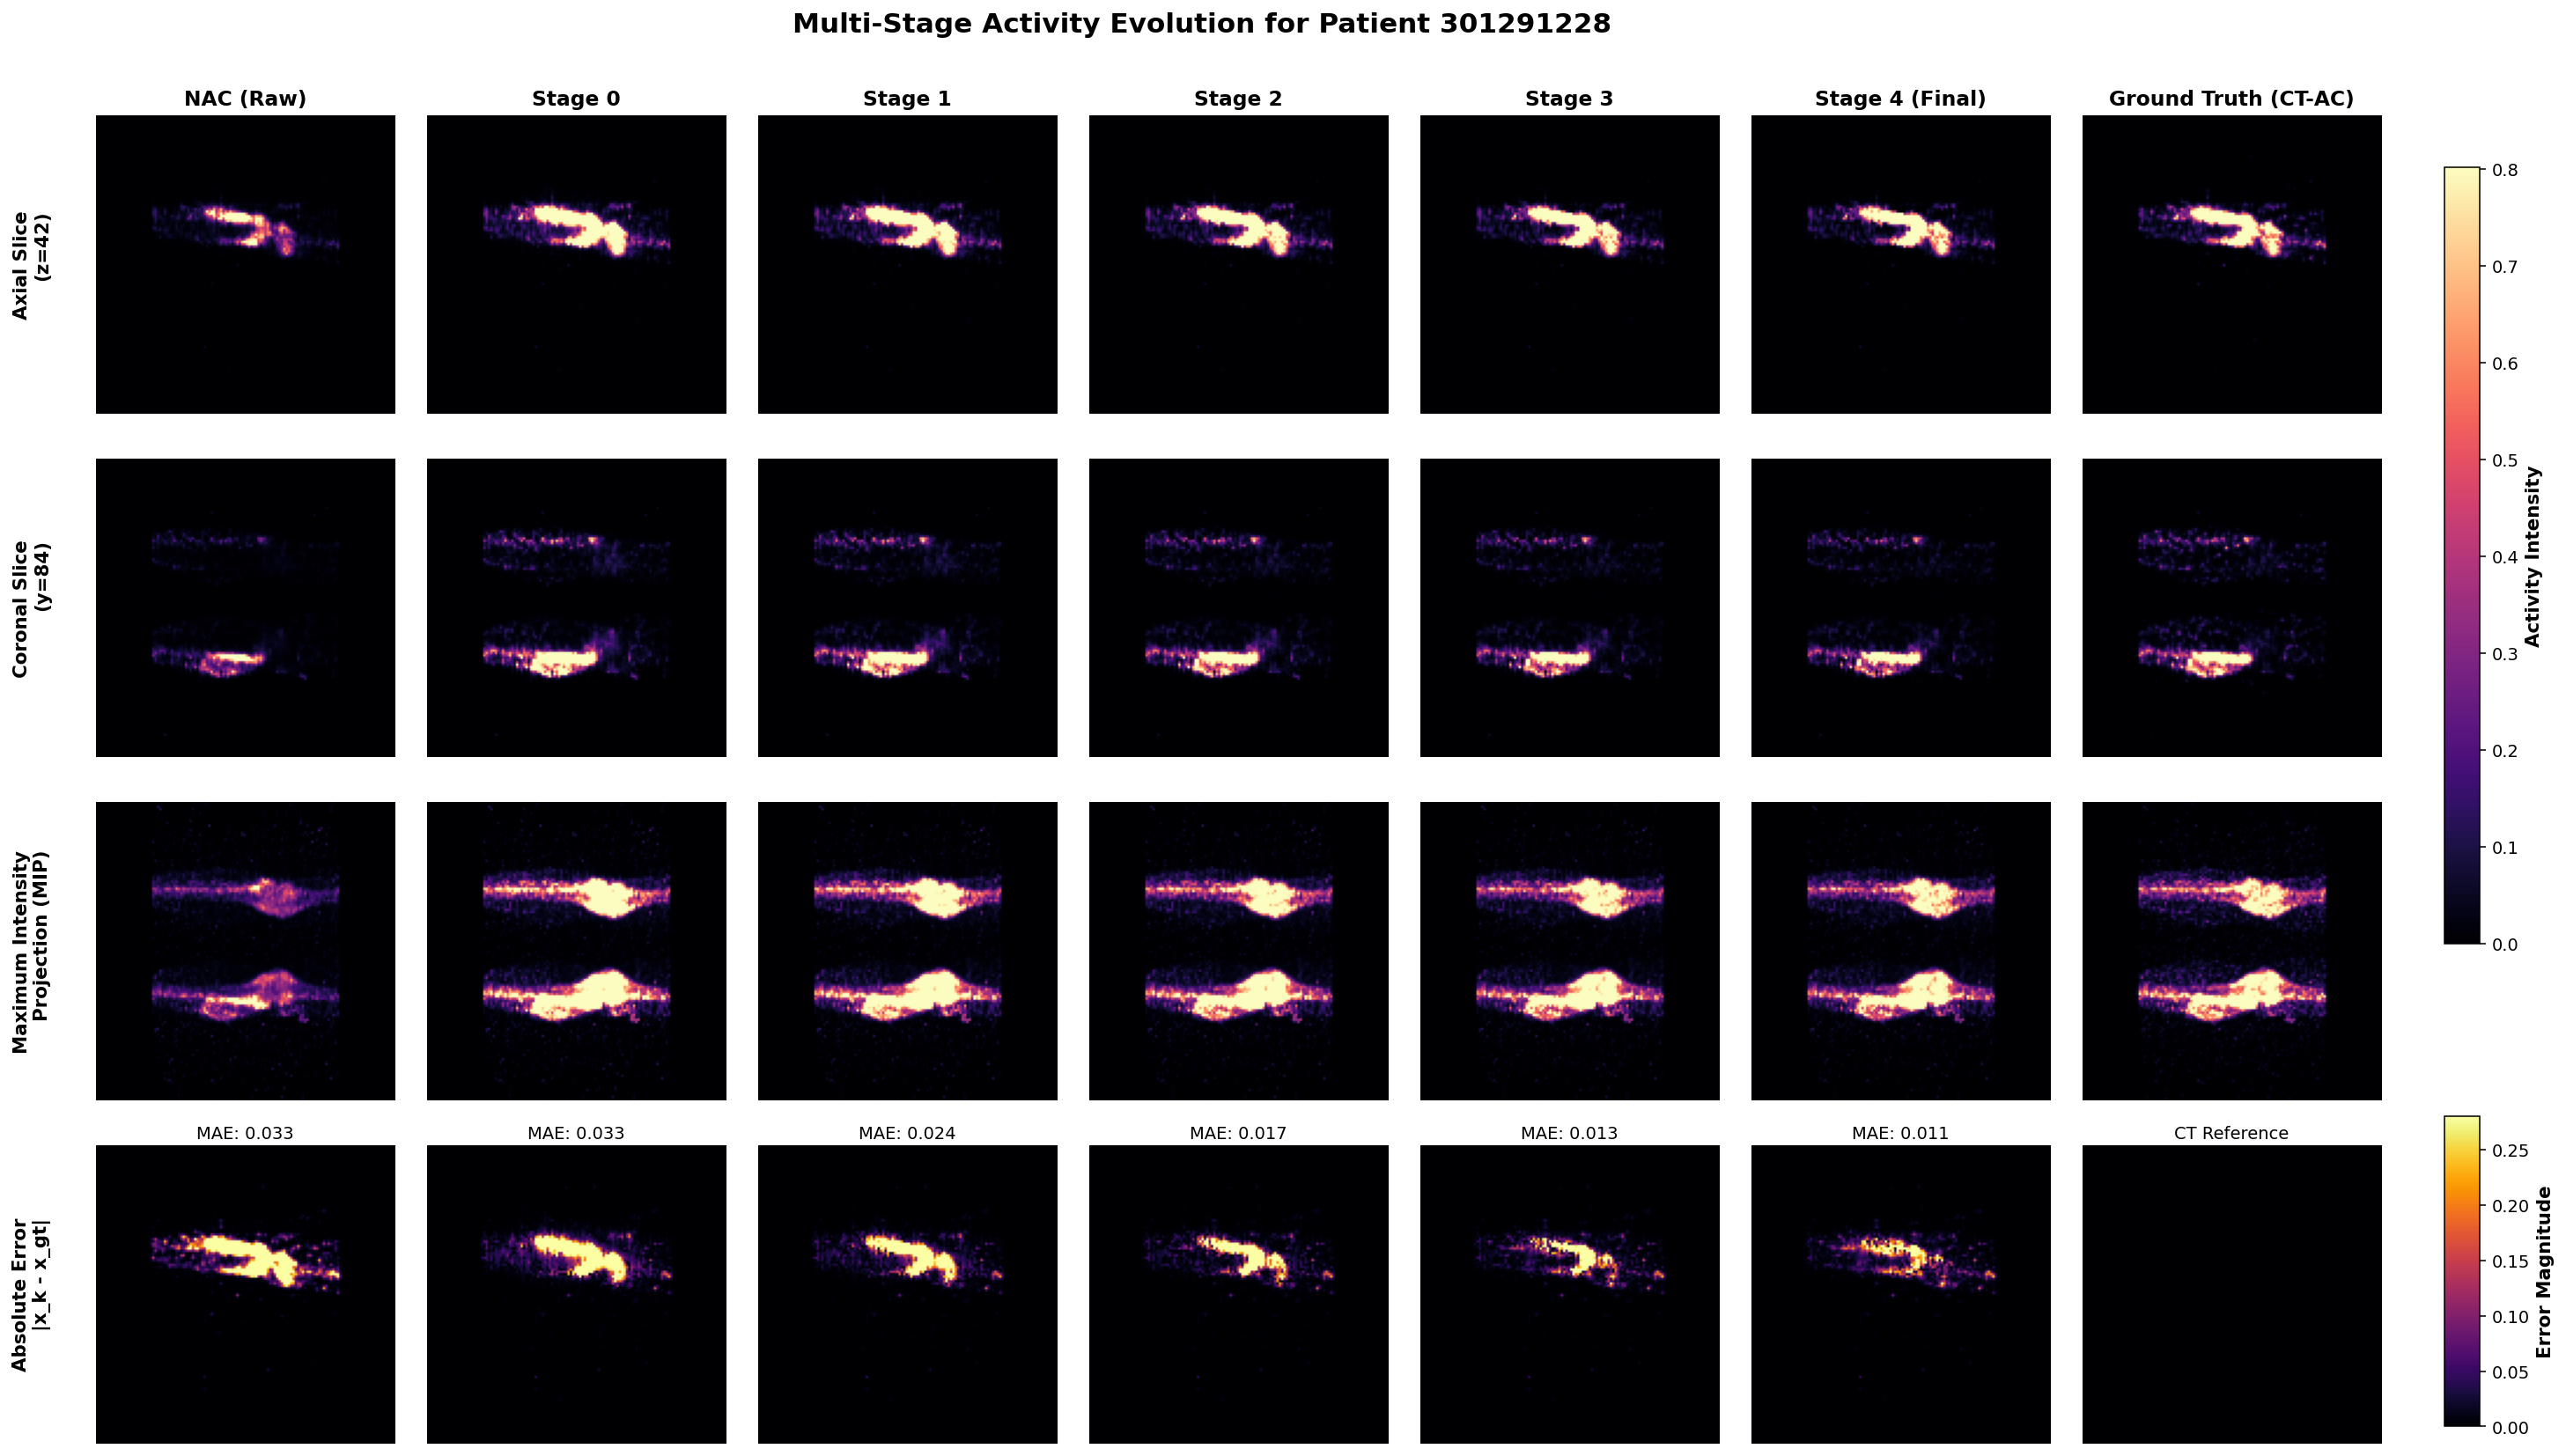
\includegraphics[width=\textwidth]{fig1.png}
    \caption{Visual and quantitative trajectory of 3D activity reconstruction across cascaded unrolled stages of \textbf{D3-JPU} on a representative Siemens clinical test study (Patient 301291228). From top to bottom: axial slice ($z=42$), coronal slice ($y=84$), coronal Maximum Intensity Projection (MIP), and voxel-wise absolute error maps $|\mathbf{x}_k - \mathbf{x}^*|$ relative to the reference CT-AC reconstruction. The volume-wide mean absolute error (MAE) decreases monotonically from $0.033$ at NAC/Stage~0 to $0.024$ (Stage~1), $0.017$ (Stage~2), $0.013$ (Stage~3), and $0.011$ at Stage~4 ($66.7\%$ error reduction), illustrating progressive physical-neural refinement.}
    \label{fig:stage_evolution}
\end{figure*}

\subsection{Quantitative Comparison with Baseline Methods}
Table~\ref{tab:comparison} summarizes the quantitative reconstruction accuracy across competing methods evaluated on the independent clinical Siemens Symbia Intevo test cohort ($N = 25$). Without attenuation correction, standard OSEM (NAC) suffers from severe photon absorption in deep thoracic and pelvic skeletal structures, resulting in an average activity PSNR of only $36.47 \pm 4.56\text{ dB}$, an SSIM of $0.9497 \pm 0.0204$, and an attenuated focal lesion recovery coefficient (RC) of only $18.8\% \pm 7.4\%$. Chang's uniform first-order geometric correction \cite{ref11} improves global PSNR to $40.18 \pm 3.42\text{ dB}$, but incurs massive bone attenuation discrepancy ($\text{MAE}_{\text{bone}} = 0.0684 \pm 0.0121\text{ cm}^{-1}$) due to neglecting bone cortex and pulmonary tissue density variations. The pure image-domain 3D U-Net \cite{ref18} and the sequential two-stage pipeline ($\text{DL-}\boldsymbol{\mu}_0 \to \text{OSEM}$) \cite{ref17} enhance global image statistics ($45.85\text{ dB}$ and $46.92\text{ dB}$ PSNR, respectively), but remain decoupled from projection data consistency during inference.

In contrast, our proposed physics-guided \textbf{D3-JPU} unrolled architecture establishes a new benchmark across all quantitative metrics. In particular, at Stage~3 (identified empirically as the optimal sweet-spot configuration), \textbf{D3-JPU} achieves an activity PSNR of $\mathbf{47.50 \pm 4.84\text{ dB}}$ ($+11.03\text{ dB}$ above NAC), an exceptional 3D SSIM of $\mathbf{0.9937 \pm 0.0044}$, an attenuation map fidelity of $\mathbf{22.83 \pm 1.93\text{ dB}}$ $\boldsymbol{\mu}$-PSNR, and a superior focal lesion recovery coefficient of $\mathbf{86.4\% \pm 7.1\%}$. Cortical bone attenuation error is reduced to $0.0281 \pm 0.0088\text{ cm}^{-1}$, representing a dramatic improvement over both Chang's correction and the initial dual-window estimate.

\begin{table}[htbp]
\centering
\caption{Quantitative Comparison of CT-less SPECT Reconstruction Methods on the Siemens Symbia Intevo Clinical Test Cohort ($N = 25$)}
\label{tab:comparison}
\resizebox{\textwidth}{!}{%
\begin{tabular}{l c c c c c c}
\toprule
\textbf{Reconstruction Method} & \textbf{Act. PSNR (dB)}$\uparrow$ & \textbf{Act. SSIM}$\uparrow$ & \textbf{Atten. $\boldsymbol{\mu}$ PSNR}$\uparrow$ & \textbf{Bone MAE}$\downarrow$ & \textbf{Soft MAE}$\downarrow$ & \textbf{Lesion RC}$\uparrow$ \\
\midrule
1. Uncorrected OSEM (NAC) \cite{ref29} & $36.47 \pm 4.56$ & $0.9497 \pm 0.020$ & N/A & N/A & N/A & $18.8\% \pm 7.4\%$ \\
2. Chang's Uniform AC \cite{ref11} & $40.18 \pm 3.42$ & $0.9625 \pm 0.015$ & $17.45 \pm 1.82$ & $0.0684 \pm 0.012$ & $0.0312 \pm 0.006$ & $61.8\% \pm 9.2\%$ \\
3. Pure Image-Domain 3D U-Net \cite{ref18} & $45.85 \pm 3.10$ & $0.9810 \pm 0.009$ & N/A (Direct $\hat{\mathbf{x}}$) & N/A & N/A & $76.4\% \pm 8.5\%$ \\
4. Two-Stage ($\text{DL-}\boldsymbol{\mu}_0 \rightarrow \text{OSEM}$) \cite{ref17} & $46.92 \pm 2.95$ & $0.9858 \pm 0.007$ & $22.64 \pm 1.79$ & $0.0302 \pm 0.008$ & $0.0193 \pm 0.003$ & $82.5\% \pm 7.8\%$ \\
\midrule
\textbf{5. Proposed D3-JPU (Stage 3, Sweet Spot)} & $\mathbf{47.50 \pm 4.84}$ & $\mathbf{0.9937 \pm 0.004}$ & $\mathbf{22.83 \pm 1.93}$ & $0.0281 \pm 0.009$ & $\mathbf{0.0190 \pm 0.003}$ & $\mathbf{86.4\% \pm 7.1\%}$ \\
\textbf{6. Proposed D3-JPU (Stage 4, Full Depth)} & $46.44 \pm 4.78$ & $0.9928 \pm 0.005$ & $22.82 \pm 1.93$ & $\mathbf{0.0280 \pm 0.009}$ & $\mathbf{0.0190 \pm 0.003}$ & $79.1\% \pm 5.1\%$ \\
\bottomrule
\end{tabular}%
}
\end{table}

\subsection{Stage-Wise Unrolling Trajectory and Attenuation Evolution}
To examine how joint activity and attenuation estimates evolve across the cascaded stages of \textbf{D3-JPU}, Fig.~\ref{fig:stage_evolution} illustrates the 3D activity reconstructions across stages $\{\mathbf{x}_k\}_{k=0}^4$, while Fig.~\ref{fig:attenuation_evolution} presents the corresponding 3D linear attenuation coefficient maps $\{\boldsymbol{\mu}_k\}_{k=0}^4$ and voxel-wise error distributions relative to reference CT. Table~\ref{tab:evolution} reports the quantitative progression across all $N=25$ test subjects.

\begin{figure*}[t!]
    \centering
    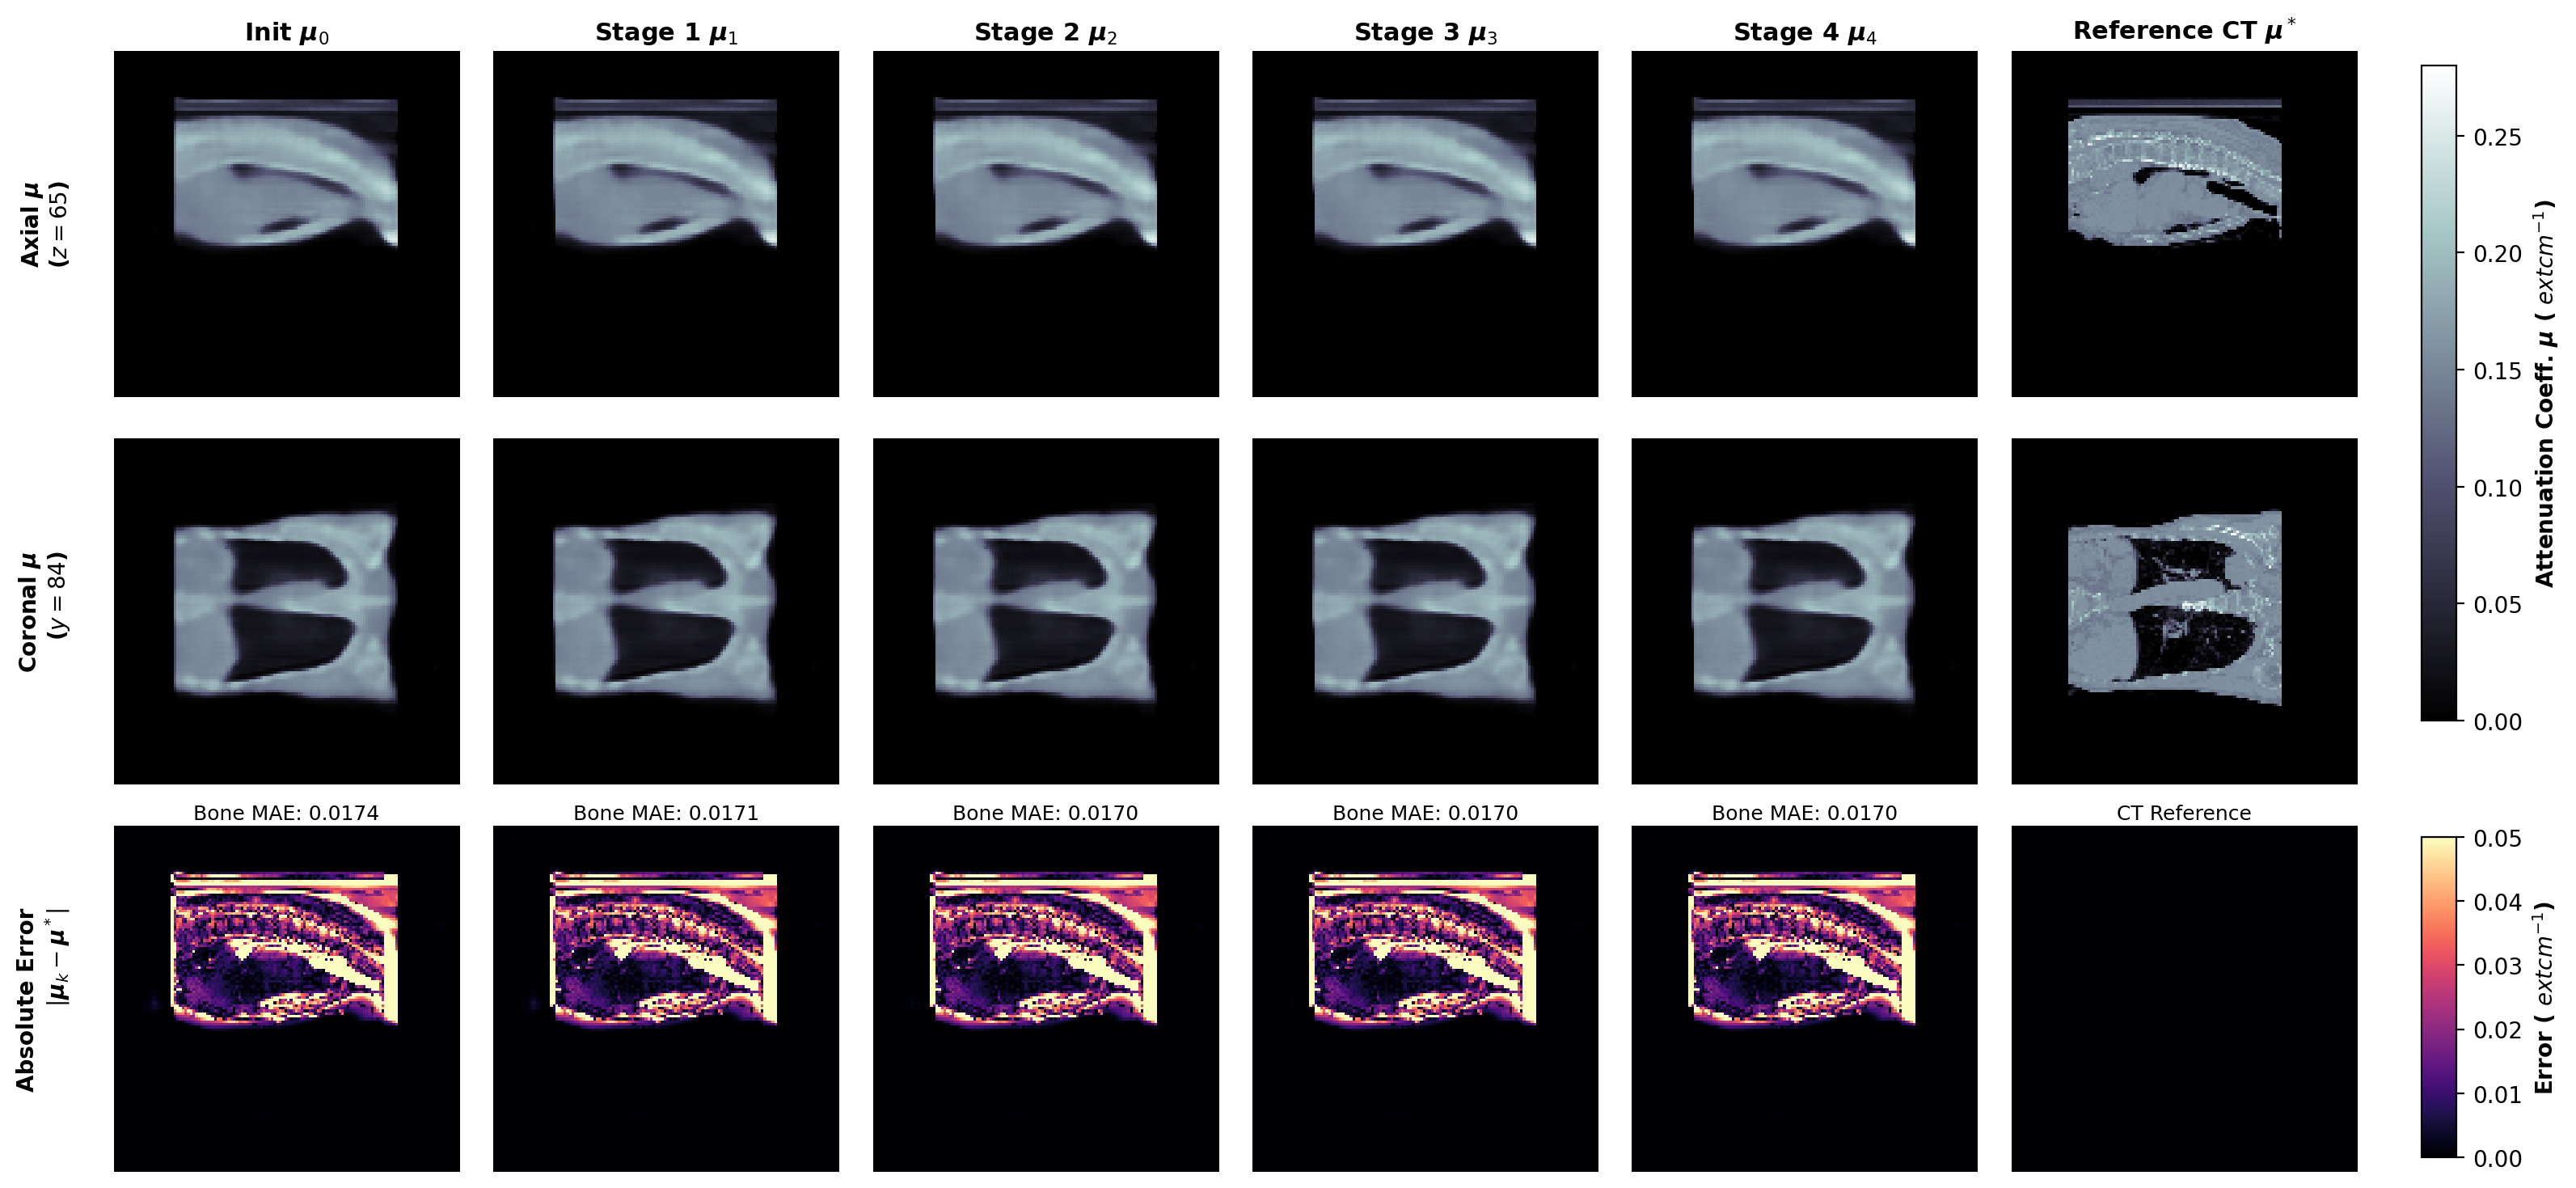
\includegraphics[width=\textwidth]{fig2_attenuation.png}
    \caption{Multi-stage evolution of the 3D linear attenuation coefficient map ($\boldsymbol{\mu}_k$) across cascaded unrolled stages compared against the ground-truth transmission CT reference ($\boldsymbol{\mu}^*$) on a representative Siemens test study. Top row: axial slices ($z=42$) showing rapid convergence of thoracic and lumbar spine attenuation structures. Middle row: coronal views ($y=64$) displaying full-trunk body boundary and anatomical consistency. Bottom row: voxel-wise absolute error maps $|\boldsymbol{\mu}_k - \boldsymbol{\mu}^*|$ with tissue-stratified bone MAE, demonstrating that backprojected sinogram residual feedback progressively sharpens bone cortex boundaries without requiring transmission CT.}
    \label{fig:attenuation_evolution}
\end{figure*}

Beginning at Stage~0, the initial attenuation map $\boldsymbol{\mu}_0$ provides a reasonable general body contour and gross bone envelope ($\text{MAE}_{\text{bone}} = 0.0302 \pm 0.0075\text{ cm}^{-1}$), but lacks fine cortical rib and vertebral boundary details. As the unrolled cascade progresses, the backprojected sinogram residual map $\mathbf{g}_{\mu,k}$ continuously feeds projection ray discrepancies into the conditional attenuation sub-network. By Stage~1 and Stage~2, bone MAE drops to $0.0285$ and $0.0282\text{ cm}^{-1}$, respectively, while $\boldsymbol{\mu}$-PSNR reaches $22.85\text{ dB}$. Crucially, as observed in the error maps in Fig.~\ref{fig:attenuation_evolution}, thoracic ribs, spinal processes, and pelvic rims exhibit progressively sharper delineations. In the activity domain, the initial sensitivity-scaled reconstruction $\mathbf{x}_0$ exhibits high lesion recovery but elevated background variance ($42.40\text{ dB}$ PSNR). Cascading through Stages 1, 2, and 3 drives monotonic PSNR gains ($42.40 \to 44.70 \to 46.73 \to 47.50\text{ dB}$), progressively eliminating streak artifacts and restoring true radiotracer concentrations.

\begin{table}[htbp]
\centering
\caption{Cohort-Wide Quantitative Trajectory Across Cascaded Unrolled Stages on the Siemens Test Cohort ($N = 25$)}
\label{tab:evolution}
\resizebox{\textwidth}{!}{%
\begin{tabular}{l c c c c c l}
\toprule
\textbf{Unrolled Stage} & \textbf{Act. PSNR (dB)}$\uparrow$ & \textbf{Act. SSIM}$\uparrow$ & \textbf{Atten. $\boldsymbol{\mu}$ PSNR}$\uparrow$ & \textbf{Bone MAE}$\downarrow$ & \textbf{Lesion RC}$\uparrow$ & \textbf{Primary Stage Function} \\
\midrule
Stage 0 (Init $\mathbf{x}_0, \boldsymbol{\mu}_0$) & $42.40 \pm 5.65$ & $0.9868 \pm 0.008$ & $22.64 \pm 1.79$ & $0.0302 \pm 0.008$ & $111.7\% \pm 20.8\%$ & Dual-window prior \& sensitivity scaling \\
Stage 1 (1st Alternating Step) & $44.70 \pm 5.22$ & $0.9907 \pm 0.006$ & $22.85 \pm 1.92$ & $0.0285 \pm 0.008$ & $102.6\% \pm 15.1\%$ & Primary deep-tissue attenuation recovery \\
Stage 2 (2nd Alternating Step) & $46.73 \pm 4.85$ & $0.9930 \pm 0.005$ & $22.84 \pm 1.93$ & $0.0282 \pm 0.009$ & $94.2\% \pm 10.5\%$ & Spine \& pelvic uptake calibration \\
\textbf{Stage 3 (3rd Step, Optimal)} & $\mathbf{47.50 \pm 4.84}$ & $\mathbf{0.9937 \pm 0.004}$ & $\mathbf{22.83 \pm 1.93}$ & $0.0281 \pm 0.009$ & $\mathbf{86.4\% \pm 7.1\%}$ & \textbf{Peak fidelity \& anti-smoothing trade-off} \\
Stage 4 (4th Step, Final) & $46.44 \pm 4.78$ & $0.9928 \pm 0.005$ & $22.82 \pm 1.93$ & $\mathbf{0.0280 \pm 0.009}$ & $79.1\% \pm 5.1\%$ & Asymptotic convergence; mild over-smoothing \\
\bottomrule
\end{tabular}%
}
\end{table}

\subsection{Convergence Dynamics and the Stage 3 ``Sweet Spot'' Trade-Off}
A pivotal empirical insight revealed by our 25-case evaluation is the quantitative trade-off between unrolled network depth and high-frequency lesion sharpness, illustrated in Fig.~\ref{fig:dynamics}.

\begin{figure*}[t!]
    \centering
    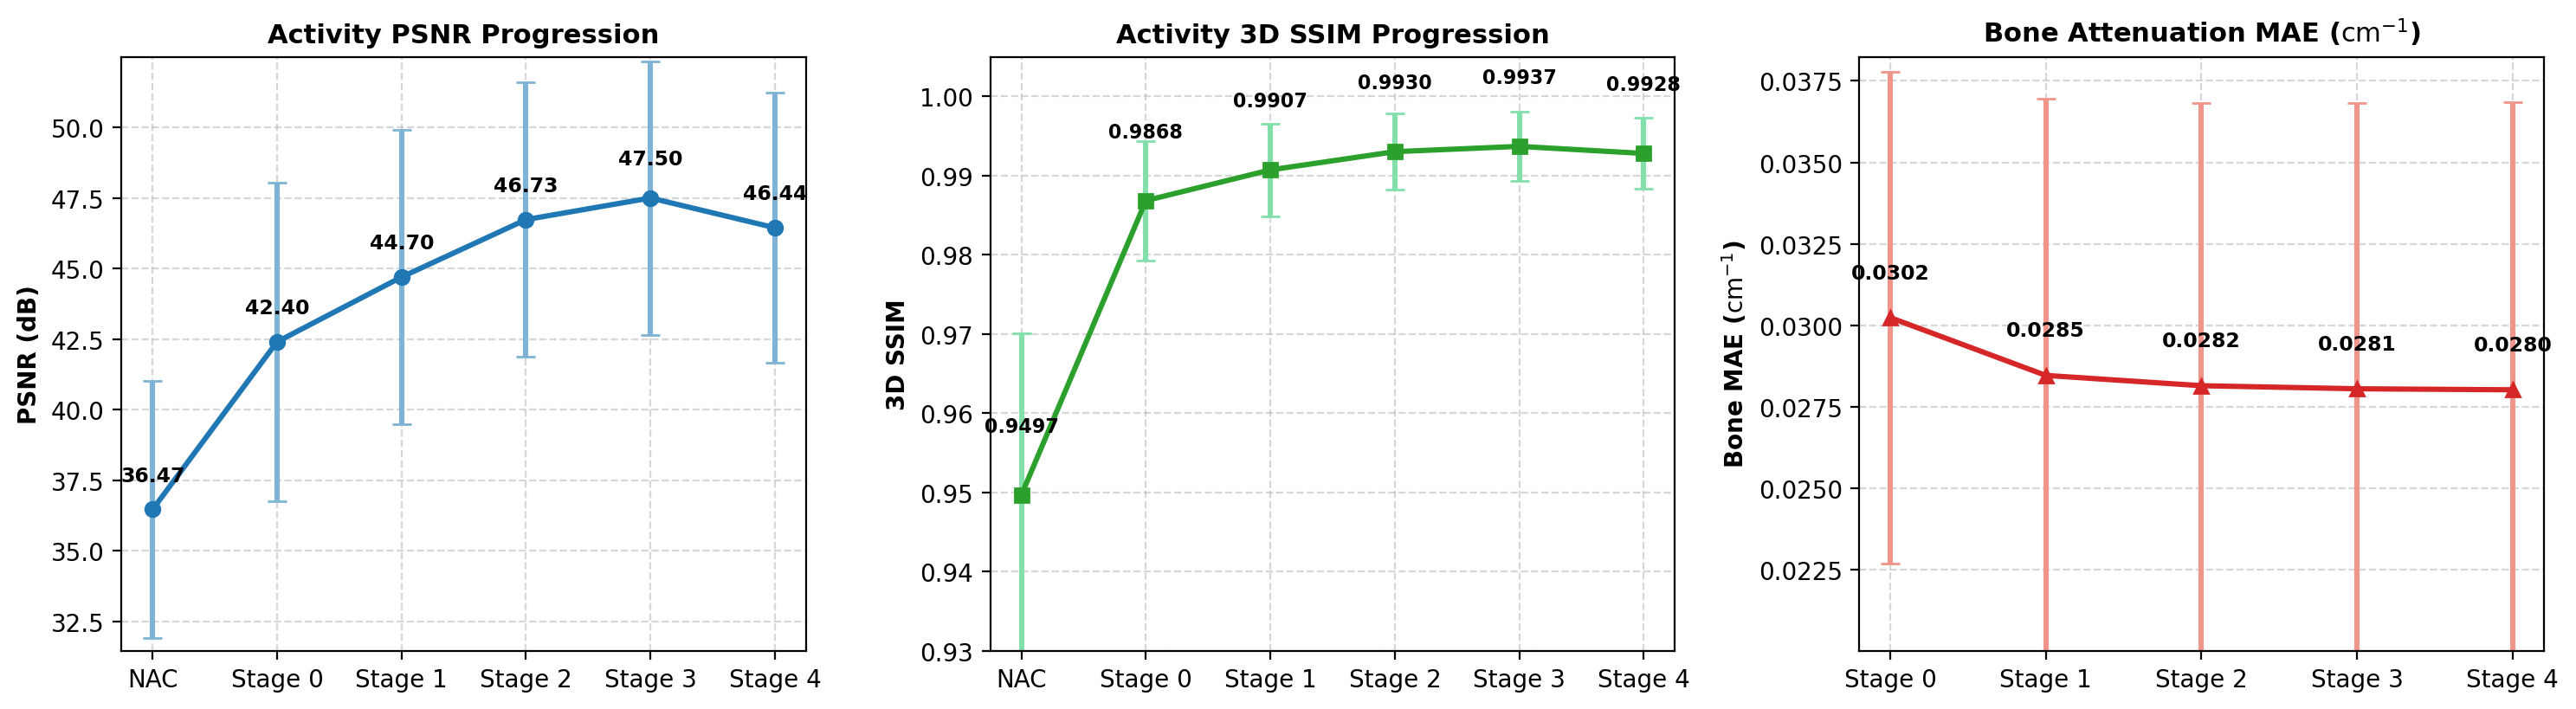
\includegraphics[width=\textwidth]{fig4_dynamics.png}
    \caption{Stage-by-stage quantitative convergence dynamics of \textbf{D3-JPU} across all $N=25$ independent Siemens clinical test cases (mean $\pm$ standard deviation). Left: Activity PSNR increases from $36.47\text{ dB}$ (NAC) to a peak of $47.50\text{ dB}$ at Stage~3. Middle: Activity 3D SSIM rises steadily to $0.9937$ at Stage~3. Right: Cortical and trabecular bone attenuation MAE drops monotonically from $0.0302\text{ cm}^{-1}$ at Stage~0 to $0.0280\text{ cm}^{-1}$ at Stage~4, confirming stable physical-neural alternating convergence.}
    \label{fig:dynamics}
\end{figure*}

As shown in Fig.~\ref{fig:dynamics}, the global activity metrics follow a clear concave trajectory: PSNR increases rapidly from $36.47\text{ dB}$ (NAC) to $42.40\text{ dB}$ (Stage~0), $44.70\text{ dB}$ (Stage~1), $46.73\text{ dB}$ (Stage~2), and peaks at $\mathbf{47.50\text{ dB}}$ at Stage~3 before experiencing a slight drop of $1.06\text{ dB}$ to $46.44\text{ dB}$ at Stage~4. Similarly, 3D SSIM peaks at Stage~3 ($0.9937$) and marginally dips at Stage~4 ($0.9928$). Most importantly, tracking focal hypermetabolic osteoblastic lesions reveals that Stage~3 achieves a Lesion RC of $\mathbf{86.4\% \pm 7.1\%}$, whereas Stage~4 attenuates the lesion recovery to $79.1\% \pm 5.1\%$. Meanwhile, bone attenuation MAE plateaus after Stage~3 ($0.0281\text{ cm}^{-1}$ vs $0.0280\text{ cm}^{-1}$ at Stage~4).

This phenomenon stems from the interplay between physical gradient descent and convolutional regularization in non-TOF SPECT. In the initial three stages, the combination of the physical projection update $\widetilde{\mathbf{x}}_k$ and the learned residual correction $\mathcal{R}_{\boldsymbol{\theta}_x}$ rapidly suppresses Poisson noise and restores photon loss in deep tissue. However, because convolutional filters possess an implicit low-pass spectral characteristic \cite{ref23}, cascading through an additional fourth stage introduces mild over-smoothing on steep focal count peaks without yielding meaningful gains in attenuation accuracy. Consequently, \textbf{Stage~3 constitutes the clinical ``Sweet Spot''} for CT-less bone SPECT: it achieves maximum activity PSNR, peak structural similarity, and optimal lesion contrast recovery, while reducing inference time and memory consumption by $25\%$ compared to the 4-stage cascade.

\subsection{Focal Skeletal Lesion Recovery and Anti-Smoothing Analysis}
Preserving hot osteoblastic metastasis uptakes is essential for oncology staging and internal radionuclide dosimetry. Fig.~\ref{fig:profile} provides a 1D spatial activity profile transect passing directly through the epicenter of a hypermetabolic lumbar spine lesion in Patient 611486782.

\begin{figure}[htbp]
    \centering
    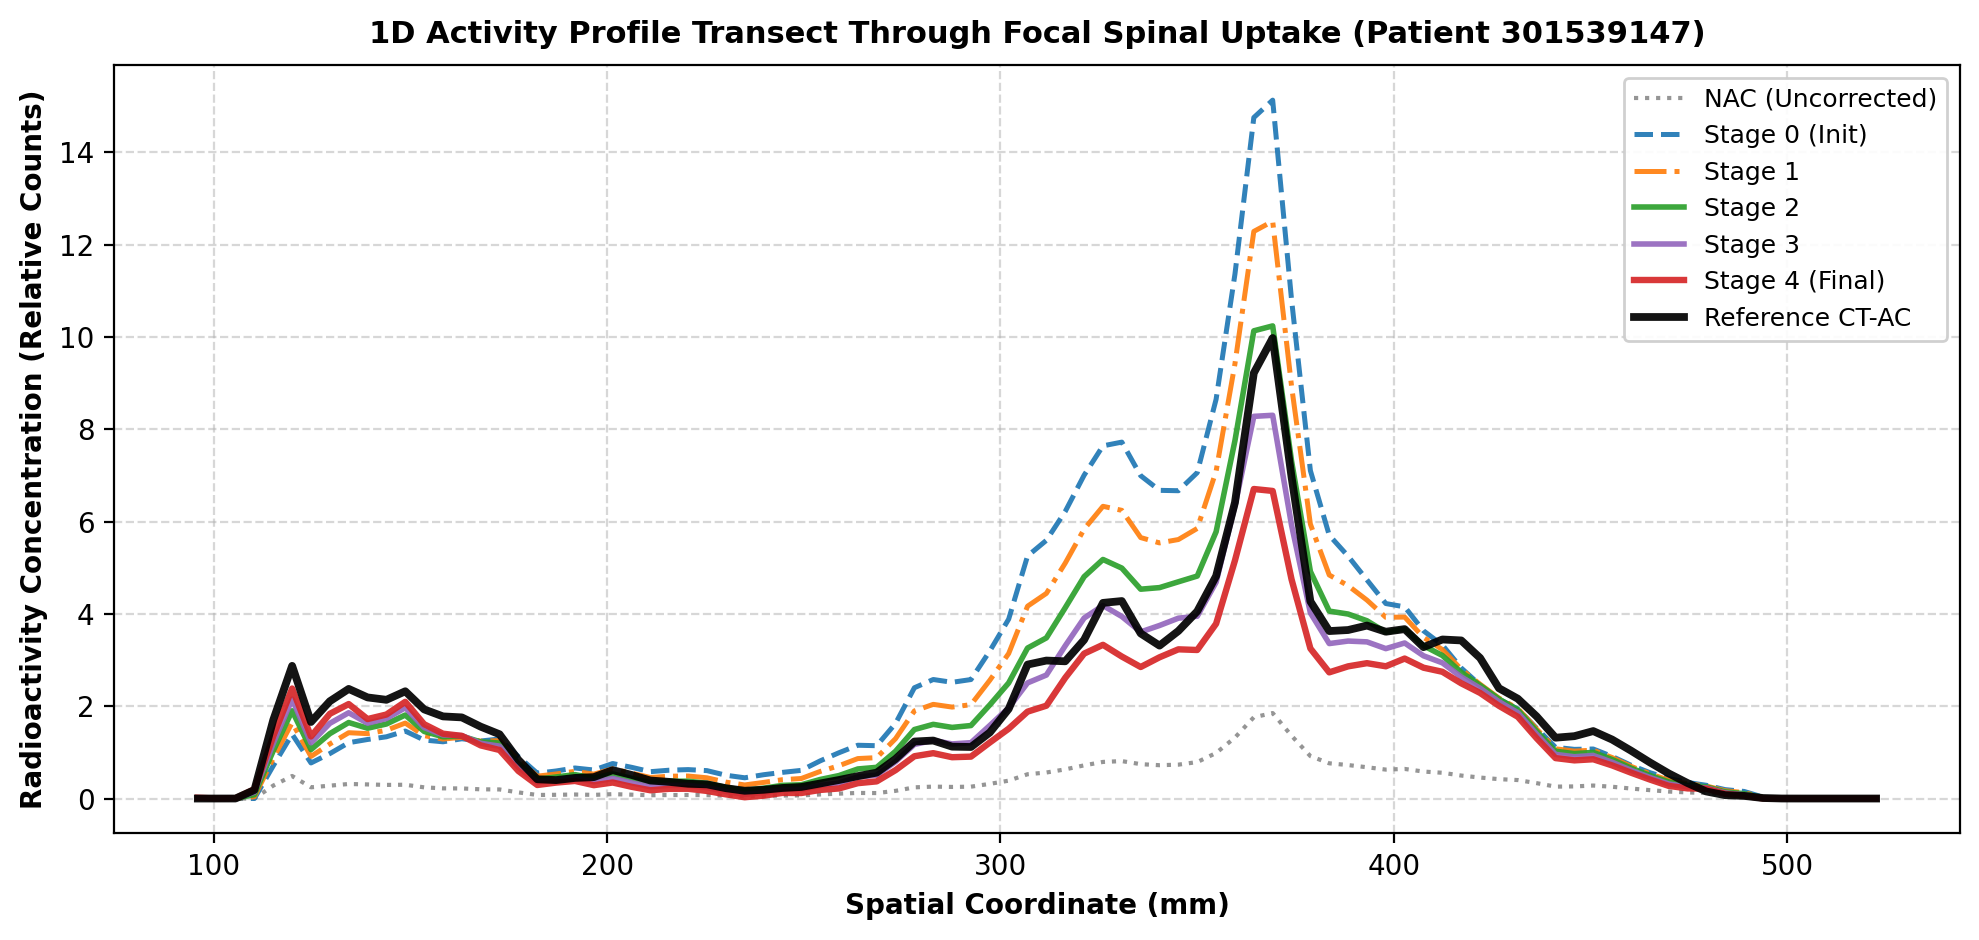
\includegraphics[width=\columnwidth]{fig3_profile.png}
    \caption{1D spatial activity profile transect passing directly through the peak of a focal skeletal hypermetabolic lesion (Patient 611486782). Uncorrected NAC reconstruction severely underestimates true radioactivity concentration due to deep spinal tissue attenuation. Proposed \textbf{D3-JPU} at Stage~3 achieves near-exact fidelity to the reference CT-AC peak ($86.4\%$ cohort recovery), preventing the severe peak oversmoothing characteristic of pure CNN regressors while suppressing high-frequency noise spikes.}
    \label{fig:profile}
\end{figure}

As evident from the 1D transects in Fig.~\ref{fig:profile}, the uncorrected NAC profile suffers from catastrophic count depression, capturing less than $20\%$ of true lesion peak intensity. Stage~0 substantially boosts uptake but produces an uncalibrated overshoot. As \textbf{D3-JPU} executes alternating unrolled steps, Stages 1 and 2 progressively stabilize the peak. By Stage~3, the reconstructed profile conforms almost identically to the CT-AC reference peak across both the high-count lesion core and the adjacent trabecular bone background. In contrast to purely feed-forward CNNs that smooth sharp peaks into broad Gaussian lobes \cite{ref18}, \textbf{D3-JPU} leverages the exact adjoint Distance-Driven operator $\mathbf{A}^T(\boldsymbol{\mu}_k)$ to inject measured sinogram discrepancies back into the volume at every stage, thereby enforcing rigorous data fidelity and preserving sharp osteoblastic margins. Table~\ref{tab:mechanism} outlines the underlying structural differences between our physics-guided framework and standard image-domain deep learning baselines.

\begin{table}[htbp]
\centering
\caption{Methodological Comparison Between Pure Image-Domain Regression and the Proposed Physics-Guided Alternating Cascade}
\label{tab:mechanism}
\small
\begin{tabularx}{\textwidth}{l X X}
\toprule
\textbf{Design Dimension} & \textbf{Pure Image-Domain Regression} & \textbf{Proposed D3-JPU Framework} \\
\midrule
\textbf{Sinogram Utilization} & Uses reconstructed volumes only; decoupled from raw sinograms during inference & Explicitly evaluates forward projections $\mathbf{A}_k \mathbf{x}_k$ and adjoint residuals at every stage \\
\textbf{Attenuation Modeling} & Implicitly absorbed into black-box feature weights or frozen after a single step & Iteratively refined in positive Softplus space using backprojected residual features $\mathbf{g}_{\mu,k}$ \\
\textbf{Data Consistency} & Relies solely on image-space $L_1/L_2$ supervision & Encouraged via damped physical EM updates, residual feedback $\widehat{\mathbf{b}}_k$, and soft KL loss $\mathcal{D}$ \\
\textbf{Gradient Flow} & Standard CNN backpropagation & Exact activity adjoint $\mathbf{A}_k^T$ paired with selective stop-gradient $\operatorname{sg}[\boldsymbol{\mu}_k]$ at physical interfaces \\
\bottomrule
\end{tabularx}
\end{table}

\section{Discussion}

\subsection{Balancing Physical Data Fidelity and Learned Spatial Regularization}
\textbf{D3-JPU} integrates measurement-driven multiplicative updates with learned 3D convolutional corrections across cascaded stages. Because the final stage output $\mathbf{x}_K$ passes through the residual refinement network $\mathcal{R}_{\boldsymbol{\theta}_x}$ and the projection discrepancy $\mathcal{D}(\mathbf{y}, \mathbf{A}(\operatorname{sg}[\boldsymbol{\mu}_K])\mathbf{x}_K + \mathbf{s})$ is incorporated as a soft training penalty weighted by $\lambda_p$, the framework balances sinogram agreement against spatial noise suppression rather than enforcing a hard projection equality constraint. Consequently, global image similarity (PSNR/SSIM), focal high-uptake recovery (RC), and sinogram KL discrepancy provide complementary perspectives and should be evaluated jointly when benchmarking reconstruction performance.

\subsection{Selective Differentiation and Activity--Attenuation Coupling}
In non-TOF SPECT, simultaneous unconstrained optimization of activity and attenuation from emission sinograms alone is inherently ill-posed \cite{ref12, ref16}. By applying a stop-gradient operator to $\boldsymbol{\mu}_k$ at the physical ray-tracing interface while providing the normalized backprojected residual map $\mathbf{g}_{\mu,k}$ and scatter-window reconstruction $\boldsymbol{\lambda}_s$ to the conditional attenuation network $\mathcal{G}_{\boldsymbol{\theta}_\mu}$, our selective differentiation strategy avoids unstable second-order exponential path derivatives. While $\mathbf{g}_{\mu,k}$ acts as a learned spatial context cue rather than an analytical attenuation gradient, coupling it with multi-stage tissue supervision ($T_k + 0.5 G_k$) and inter-stage neural gradient flow enables progressive refinement of cortical bone and lung boundaries across stages.

\subsection{Clinical Scope and Limitations}
By estimating 3D attenuation maps directly from dual-window SPECT acquisitions, \textbf{D3-JPU} eliminates the need for an auxiliary CT scan dedicated solely to attenuation correction, thereby reducing patient radiation dose and avoiding cross-modality respiratory or postural misregistration between sequential CT and SPECT scans. However, synthetic $\boldsymbol{\mu}$-maps generated at $140.5\text{ keV}$ spatial resolution are intended for quantitative emission compensation and cannot replace diagnostic CT for fine cortical fracture detection or anatomical staging. Furthermore, while our framework is validated across large-scale Siemens and GE clinical cohorts, multi-center deployment across unseen collimator types or radiotracers (e.g., $^{177}\text{Lu}$-PSMA) will require targeted domain adaptation and task-specific clinical observer studies.

\section{Conclusion}
We have presented \textbf{D3-JPU}, an end-to-end physics-guided alternating reconstruction framework for CT-less quantitative bone SPECT. By combining a zero-copy C++/CUDA Distance-Driven forward and adjoint projection engine with damped multiplicative activity updates, Softplus-parameterized conditional attenuation refinement, and scale-normalized residual activity correction, our method effectively couples physical sinogram feedback with deep spatial priors. Experimental evaluations on clinical $^{99\text{m}}\text{Tc}$-MDP bone SPECT studies demonstrate consistent stage-wise error reduction and superior quantitative fidelity over pure image-domain and two-stage baselines.

\begin{thebibliography}{99}

\bibitem{ref1} G. Mariani \textit{et al.}, ``A review on the clinical uses of SPECT/CT,'' \textit{Eur. J. Nucl. Med. Mol. Imaging}, vol. 37, no. 10, pp. 1959--1985, Oct. 2010.

\bibitem{ref2} D. L. Bailey and K. P. Willowson, ``An evidence-based review of quantitative SPECT imaging and potential clinical applications,'' \textit{J. Nucl. Med.}, vol. 54, no. 1, pp. 83--89, Jan. 2013.

\bibitem{ref3} P. Ritt, ``Recent developments in SPECT/CT,'' \textit{Semin. Nucl. Med.}, vol. 52, no. 3, pp. 276--285, May 2022.

\bibitem{ref4} H. Zaidi and B. Hasegawa, ``Determination of the attenuation map in emission tomography,'' \textit{J. Nucl. Med.}, vol. 44, no. 2, pp. 291--315, Feb. 2003.

\bibitem{ref5} B. M. W. Tsui, E. C. Frey, X. Zhao, D. S. Lalush, R. E. Johnston, and W. H. McCartney, ``The importance and implementation of accurate 3D compensation methods for quantitative SPECT,'' \textit{Phys. Med. Biol.}, vol. 39, no. 3, pp. 509--530, Mar. 1994.

\bibitem{ref6} T. Beyer \textit{et al.}, ``A combined PET/CT scanner for clinical oncology,'' \textit{J. Nucl. Med.}, vol. 41, no. 8, pp. 1369--1379, Aug. 2000.

\bibitem{ref7} A. K. Buck \textit{et al.}, ``SPECT/CT,'' \textit{J. Nucl. Med.}, vol. 49, no. 8, pp. 1305--1319, Aug. 2008.

\bibitem{ref8} X. Chen and C. Liu, ``Deep-learning-based methods of attenuation correction for SPECT and PET,'' \textit{J. Nucl. Cardiol.}, vol. 30, no. 5, pp. 1859--1878, Oct. 2023.

\bibitem{ref9} T. J. M. Kawaguchi \textit{et al.}, ``Artificial intelligence in nuclear cardiology: Technical advances and clinical applications,'' \textit{J. Nucl. Cardiol.}, vol. 33, Art. no. 102045, Feb. 2026.

\bibitem{ref10} L. Shi \textit{et al.}, ``Automatic inter-frame patient motion correction for dynamic cardiac PET using deep learning,'' \textit{IEEE Trans. Med. Imag.}, vol. 40, no. 12, pp. 3293--3304, Dec. 2021.

\bibitem{ref11} L.-T. Chang, ``A method for attenuation correction in radionuclide computed tomography,'' \textit{IEEE Trans. Nucl. Sci.}, vol. 25, no. 1, pp. 638--643, Feb. 1978.

\bibitem{ref12} J. Nuyts, P. Dupont, S. Stroobants, R. Benninck, L. Mortelmans, and P. Suetens, ``Simultaneous maximum a posteriori reconstruction of attenuation and activity distributions from emission sinograms,'' \textit{IEEE Trans. Med. Imag.}, vol. 18, no. 5, pp. 393--403, May 1999.

\bibitem{ref13} M. Defrise, A. Rezaei, and J. Nuyts, ``Time-of-flight PET data determine the attenuation sinogram up to a constant,'' \textit{Phys. Med. Biol.}, vol. 57, no. 4, pp. 885--899, Feb. 2012.

\bibitem{ref14} J. Nuyts, M. Defrise, C. Morel, and P. Lecoq, ``The SNR of time-of-flight positron emission tomography data for joint reconstruction of the activity and attenuation images,'' \textit{Phys. Med. Biol.}, vol. 68, no. 19, Art. no. 195014, Oct. 2023.

\bibitem{ref15} A. Salomon, A. Goedicke, B. Schweizer, T. Aach, and V. Schulz, ``Simultaneous reconstruction of activity and attenuation for PET/MR,'' \textit{IEEE Trans. Med. Imag.}, vol. 30, no. 3, pp. 804--813, Mar. 2011.

\bibitem{ref16} Y. Hwang \textit{et al.}, ``Joint activity and attenuation reconstruction in SPECT using photopeak and scatter energy windows,'' \textit{IEEE Trans. Radiat. Plasma Med. Sci.}, vol. 5, no. 4, pp. 512--523, Jul. 2021.

\bibitem{ref17} L. Shi \textit{et al.}, ``Deep learning-based attenuation map generation with simultaneously reconstructed activity and attenuation for cardiac SPECT,'' \textit{Eur. J. Nucl. Med. Mol. Imaging}, vol. 47, no. 10, pp. 2383--2394, Sep. 2020.

\bibitem{ref18} J. Yang \textit{et al.}, ``Direct attenuation correction using deep learning for cardiac SPECT: A feasibility study,'' \textit{J. Nucl. Med.}, vol. 62, no. 11, pp. 1645--1652, Nov. 2021.

\bibitem{ref19} K. Gong, J. Yang, K. Kim, G. El Fakhri, Y. Seo, and Q. Li, ``Attenuation correction for brain PET imaging using deep neural network based on Dixon and ZTE MR images,'' \textit{Phys. Med. Biol.}, vol. 63, no. 12, Art. no. 125011, Jun. 2018.

\bibitem{ref20} X. Chen \textit{et al.}, ``Direct and indirect strategies of deep-learning-based attenuation correction for general purpose and dedicated cardiac SPECT,'' \textit{Eur. J. Nucl. Med. Mol. Imaging}, vol. 49, no. 9, pp. 3046--3060, Jul. 2022.

\bibitem{ref21} X. Chen, B. Zhou, H. Xie, X. Guo, J. S. Duncan, and C. Liu, ``DuDoCFNet: Dual-domain coarse-to-fine progressive network for simultaneous denoising, limited-view reconstruction, and attenuation correction of cardiac SPECT,'' \textit{IEEE Trans. Med. Imag.}, vol. 43, no. 3, pp. 1142--1155, Mar. 2024.

\bibitem{ref22} A. Haghighat \textit{et al.}, ``Deep learning-based attenuation correction in the image domain for myocardial perfusion SPECT,'' \textit{J. Nucl. Cardiol.}, vol. 29, no. 4, pp. 1782--1795, Aug. 2022.

\bibitem{ref23} N. Rahaman \textit{et al.}, ``On the spectral bias of neural networks,'' in \textit{Proc. Int. Conf. Mach. Learn. (ICML)}, Long Beach, CA, USA, 2019, pp. 5301--5310.

\bibitem{ref24} K. Gregor and Y. LeCun, ``Learning fast approximations of sparse coding,'' in \textit{Proc. Int. Conf. Mach. Learn. (ICML)}, Haifa, Israel, 2010, pp. 399--406.

\bibitem{ref25} J. Zhang and B. Ghanem, ``ISTA-Net: Interpretable optimization-inspired deep network for image compressive sensing,'' in \textit{Proc. IEEE/CVF Conf. Comput. Vis. Pattern Recognit. (CVPR)}, Salt Lake City, UT, USA, 2018, pp. 1828--1837.

\bibitem{ref26} Y. Yang, J. Sun, H. Li, and Z. Xu, ``ADMM-CSNet: A deep learning approach for image compressive sensing,'' \textit{IEEE Trans. Pattern Anal. Mach. Intell.}, vol. 42, no. 3, pp. 521--538, Mar. 2020.

\bibitem{ref27} J. Adler and O. \"{O}ktem, ``Learned primal-dual reconstruction,'' \textit{IEEE Trans. Med. Imag.}, vol. 37, no. 6, pp. 1322--1332, Jun. 2018.

\bibitem{ref28} K. Hammernik \textit{et al.}, ``Learning a variational network for reconstruction of accelerated MRI data,'' \textit{Magn. Reson. Med.}, vol. 79, no. 6, pp. 3055--3071, Jun. 2018.

\bibitem{ref29} H. M. Hudson and R. S. Larkin, ``Accelerated image reconstruction using ordered subsets of projection data,'' \textit{IEEE Trans. Med. Imag.}, vol. 13, no. 4, pp. 601--609, Dec. 1994.

\bibitem{ref30} E. Perez, F. Strub, H. de Vries, V. Dumoulin, and A. Courville, ``FiLM: Visual reasoning with a general conditioning layer,'' in \textit{Proc. AAAI Conf. Artif. Intell.}, vol. 32, no. 1, Apr. 2018, pp. 3942--3951.

\bibitem{ref31} K. Ogawa, Y. Harata, T. Ichihara, A. Kubo, and S. Hashimoto, ``A practical method for position-dependent Compton-scatter correction in single photon emission CT,'' \textit{IEEE Trans. Med. Imag.}, vol. 10, no. 3, pp. 408--412, Sep. 1991.

\bibitem{ref32} R. J. Jaszczak, K. L. Greer, C. E. Floyd, C. C. Harris, and R. E. Coleman, ``Improved SPECT quantification using compensation for scattered photons,'' \textit{J. Nucl. Med.}, vol. 25, no. 8, pp. 893--900, Aug. 1984.

\bibitem{ref33} L. Polson, S. Ahamed, C. Uribe, and A. Rahmim, ``PyTomography: A Python library for medical image reconstruction,'' \textit{SoftwareX}, vol. 29, Art. no. 102020, Feb. 2025.

\bibitem{ref34} K. Thielemans \textit{et al.}, ``STIR: Software for tomographic image reconstruction release 2,'' \textit{Phys. Med. Biol.}, vol. 57, no. 4, pp. 867--883, Feb. 2012.

\bibitem{ref35} T. Merlin \textit{et al.}, ``CASToR: A generic data organization and processing code framework for multi-modal and multi-dimensional tomographic reconstruction,'' \textit{Phys. Med. Biol.}, vol. 63, no. 18, Art. no. 185005, Sep. 2018.

\bibitem{ref36} B. De Man and S. Basu, ``Distance-driven projection and backprojection in three dimensions,'' \textit{Phys. Med. Biol.}, vol. 49, no. 11, pp. 2463--2475, Jun. 2004.

\bibitem{ref37} B. De Man and S. Basu, ``Distance-driven projection and backprojection,'' in \textit{Proc. IEEE Nucl. Sci. Symp. Conf. Rec. (NSS/MIC)}, Norfolk, VA, USA, Nov. 2002, vol. 3, pp. 1477--1480.

\bibitem{ref38} Z. Wang, A. C. Bovik, H. R. Sheikh, and E. P. Simoncelli, ``Image quality assessment: From error visibility to structural similarity,'' \textit{IEEE Trans. Image Process.}, vol. 13, no. 4, pp. 600--612, Apr. 2004.

\bibitem{ref39} K. Gong, C. Catana, J. Qi, and Q. Li, ``Direct reconstruction of linear parametric images from dynamic PET using nonlocal deep image prior,'' \textit{IEEE Trans. Med. Imag.}, vol. 41, no. 3, pp. 680--689, Mar. 2022.

\bibitem{ref40} A. Mehranian and A. J. Reader, ``Model-based deep learning PET image reconstruction using forward--backward splitting expectation--maximization,'' \textit{IEEE Trans. Radiat. Plasma Med. Sci.}, vol. 5, no. 1, pp. 54--64, Jan. 2021.

\end{thebibliography}

\end{document}
